\documentclass[12pt]{article}
\usepackage{enumerate}
\usepackage{mathematics}

\DeclareMathOperator{\id}{\mathrm{id}}


\begin{document}

\section{Exercises in lecture notes}

\begin{mdframed}
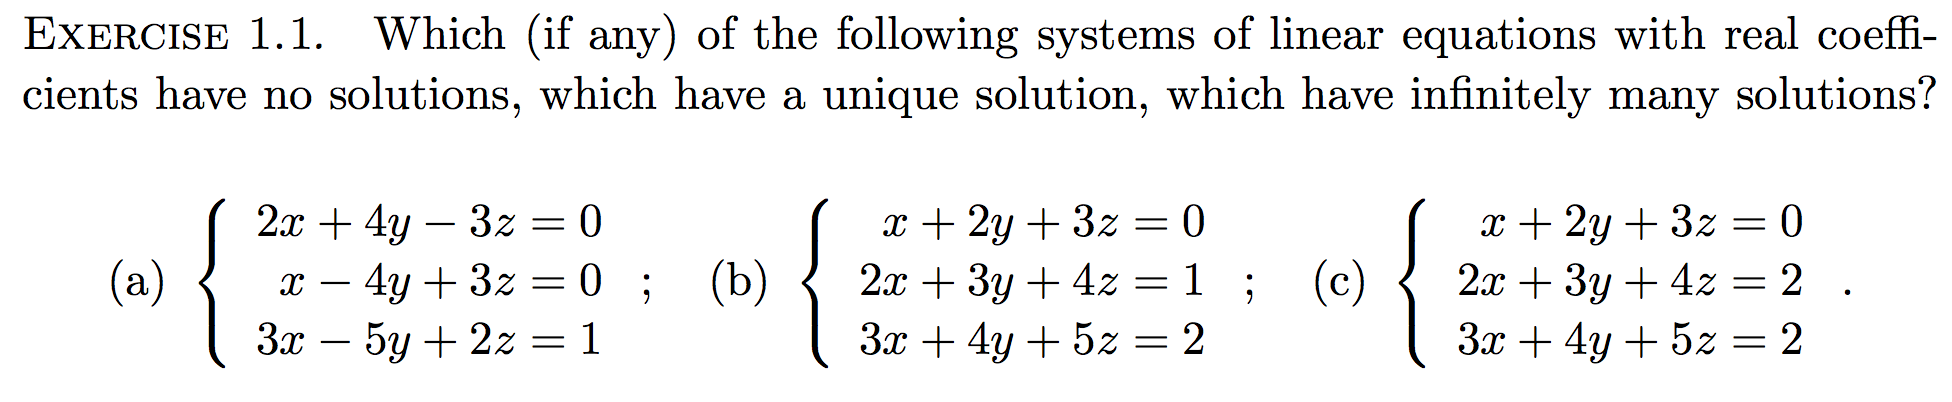
\includegraphics[width=400pt]{img/oxford-prelims-M1-linear-algebra-1-1.png}
\end{mdframed}
\begin{enumerate}[label=(\alph*)]
\item
  \begin{align*}
    \matMMMxNNN{2}{~~4}{-3}
               {1}{-4}{~~3}
               {3}{-5}{~~2} \vecMMM{x}{y}{z} = \vecMMM{0}{0}{1}\\
    ~\\
    \begin{amatrix}{3}
      2 & ~~4 &   -3  & 0\\
      1 &  -4 &  ~~3  & 0\\
      3 &  -5 &  ~~2  & 1
    \end{amatrix}&
                        ~\\
                        ~\\
    \begin{amatrix}{3}
      2 & ~~4 &   -3  & 0\\
      0 &  -22 &  ~~13  & 2\\
      0 &  -12 &  ~~9  & 0\\
    \end{amatrix}&
  \end{align*}
\end{enumerate}

\begin{mdframed}
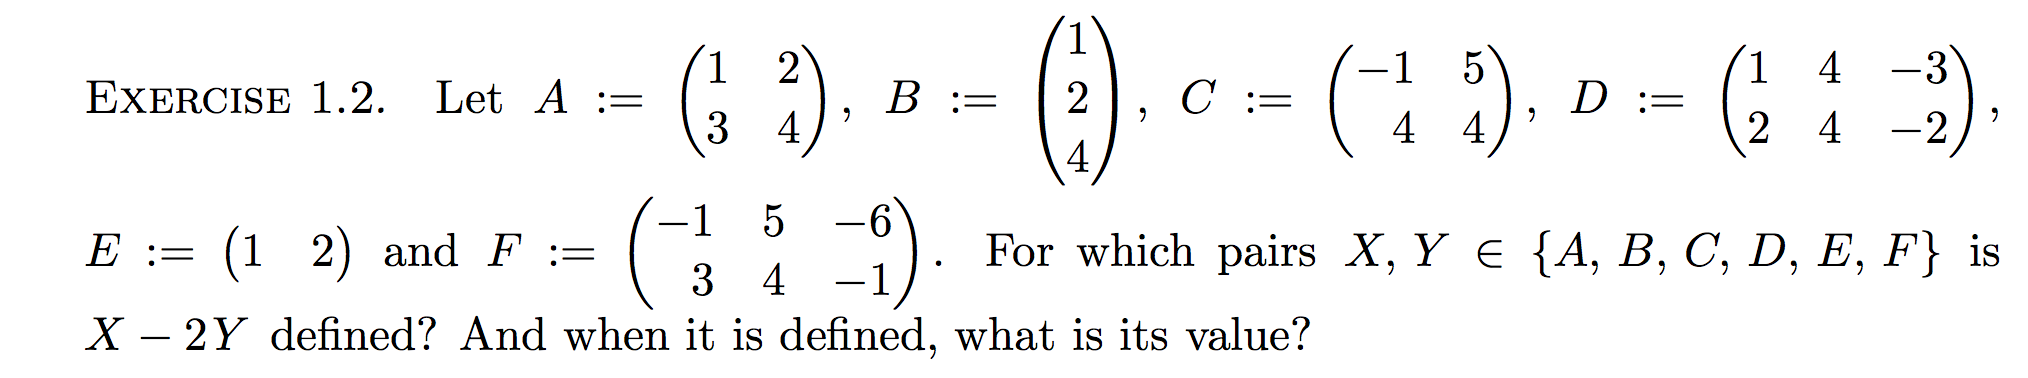
\includegraphics[width=400pt]{img/oxford-prelims-M1-linear-algebra-1-2.png}
\end{mdframed}

\begin{mdframed}
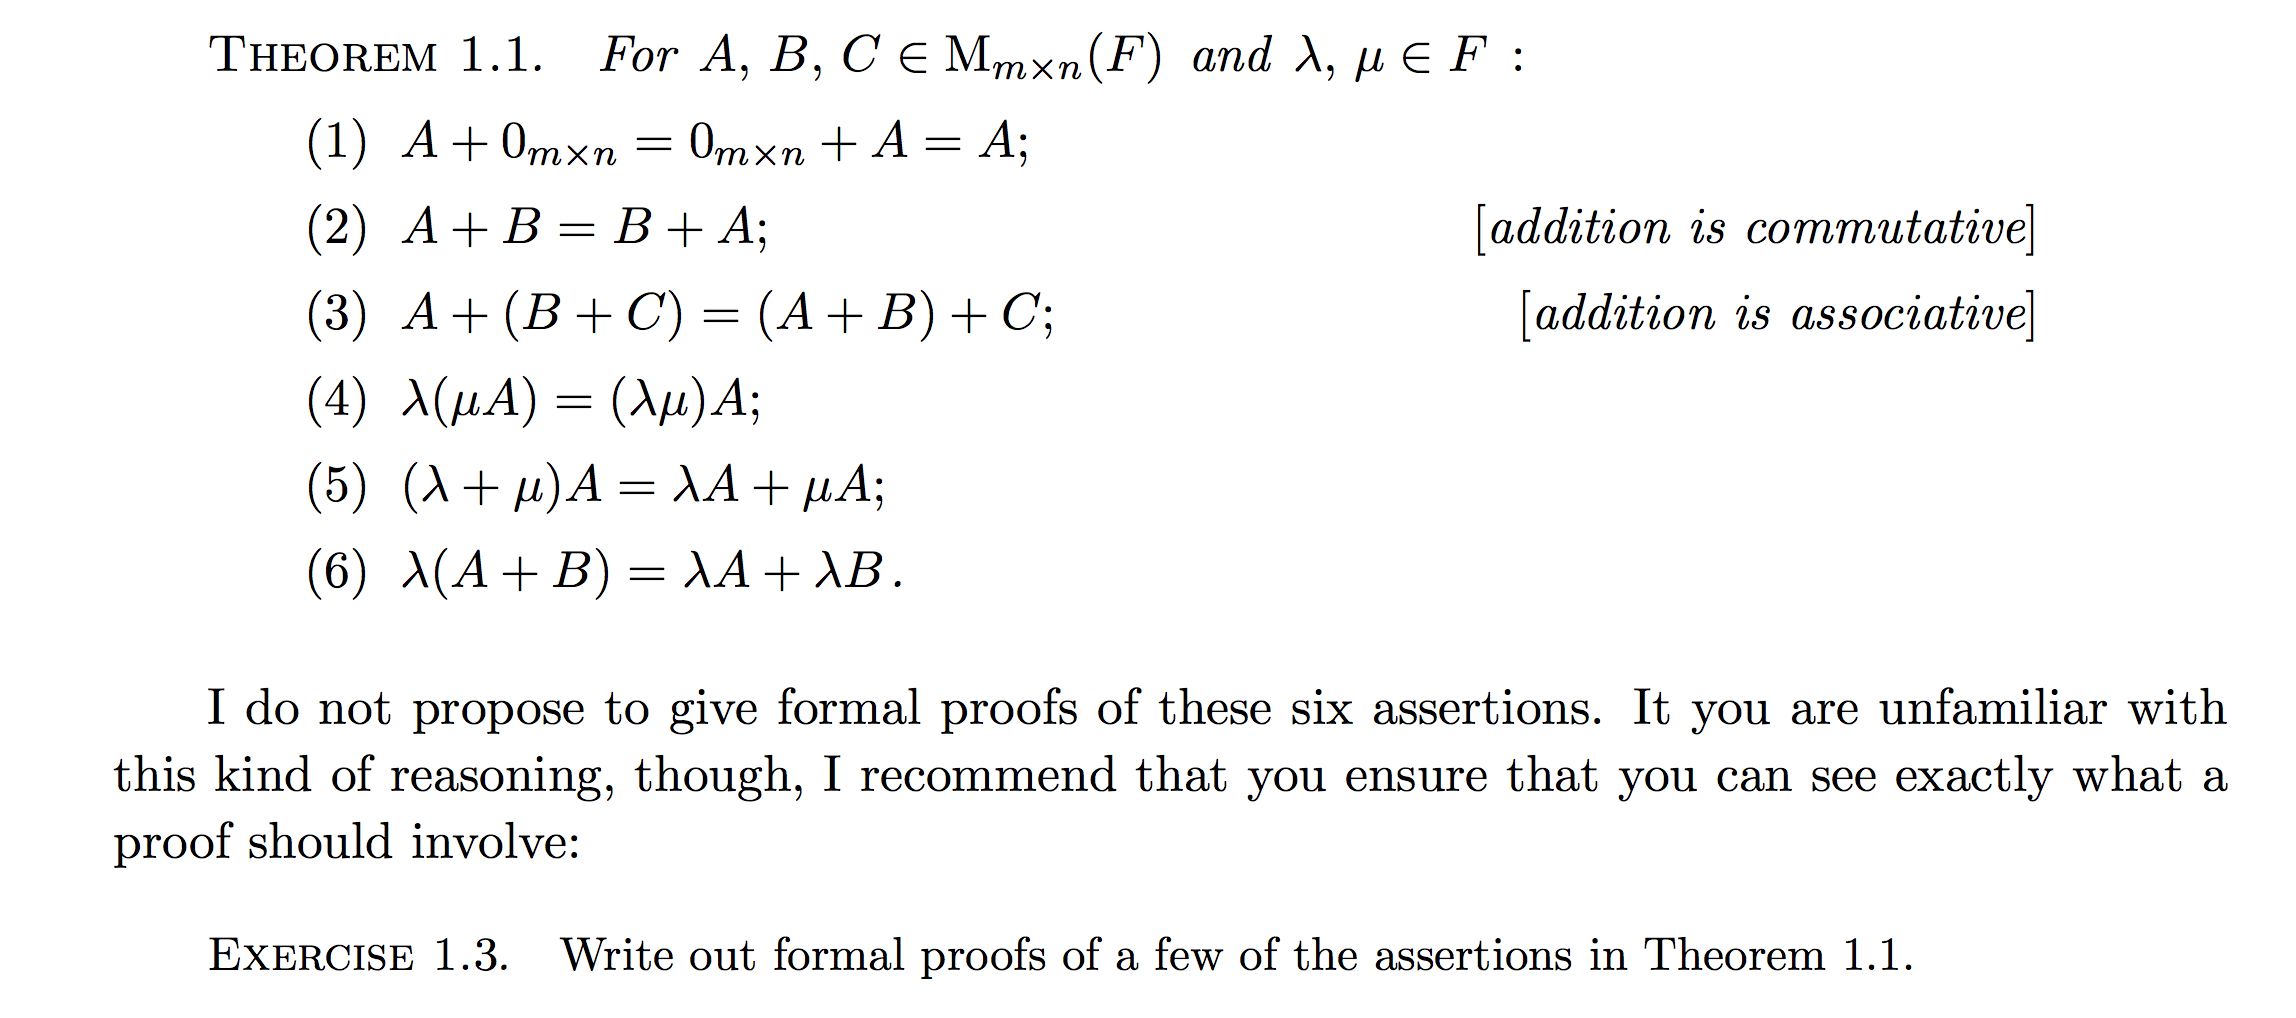
\includegraphics[width=400pt]{img/oxford-prelims-M1-linear-algebra-1-3.png}
\end{mdframed}

\begin{mdframed}
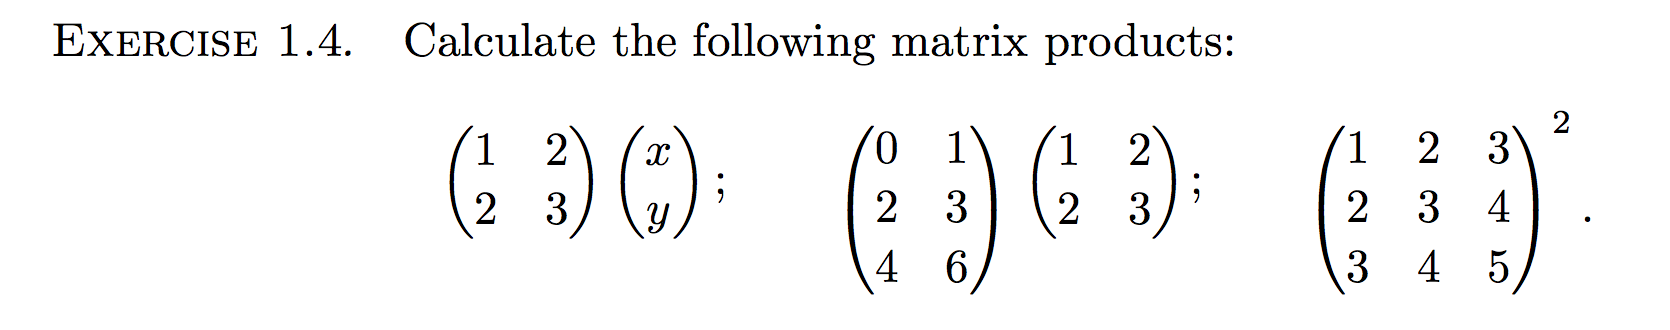
\includegraphics[width=400pt]{img/oxford-prelims-M1-linear-algebra-1-4.png}
\end{mdframed}

\begin{mdframed}
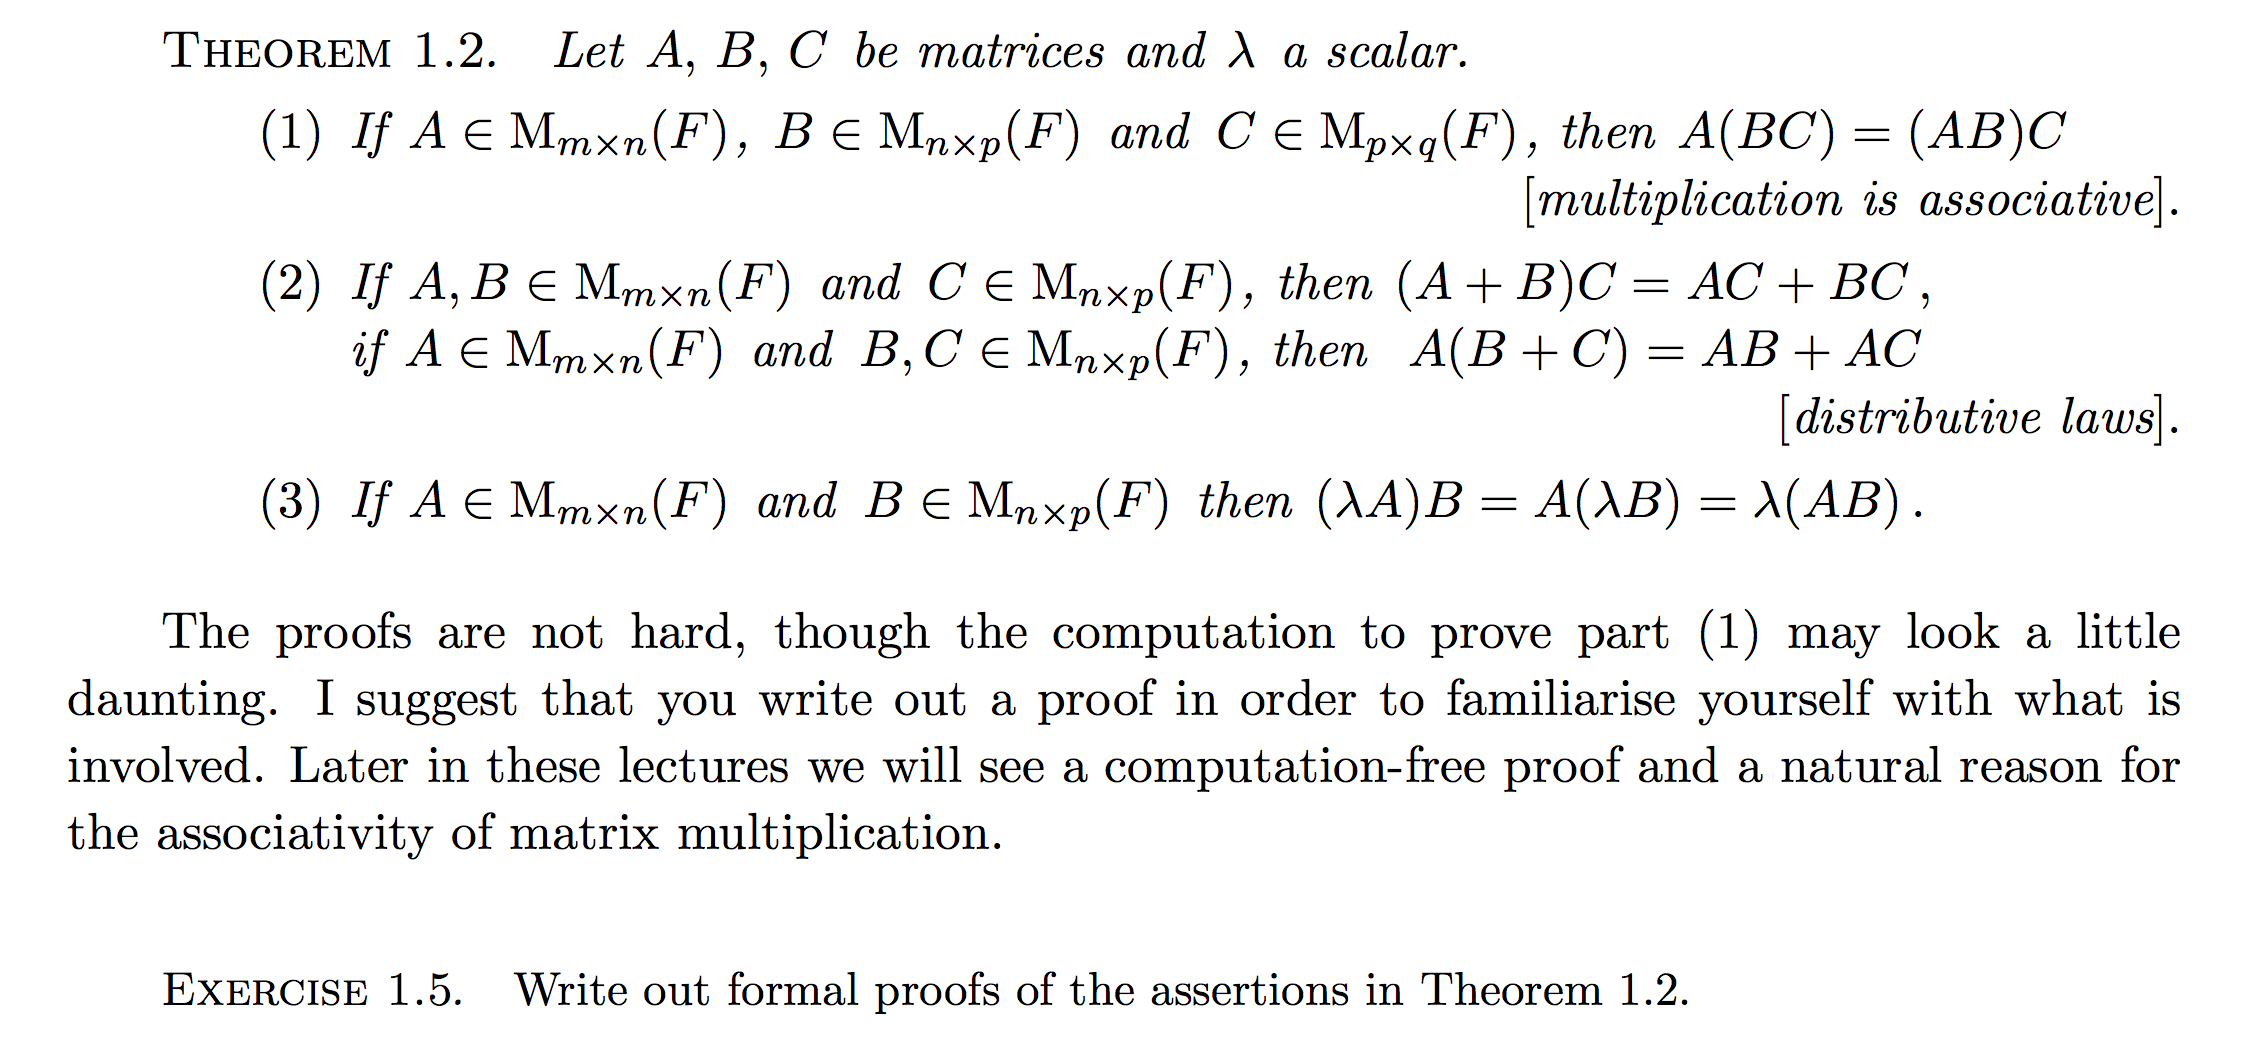
\includegraphics[width=400pt]{img/oxford-prelims-M1-linear-algebra-1-5.png}
\end{mdframed}

\begin{mdframed}
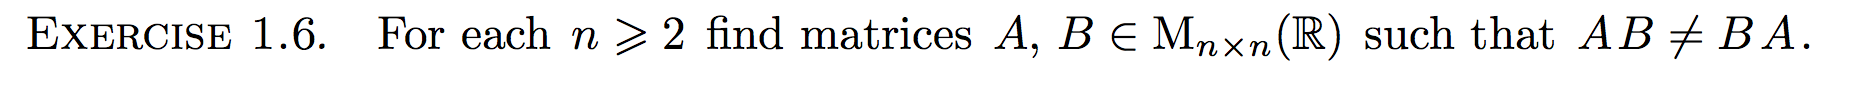
\includegraphics[width=400pt]{img/oxford-prelims-M1-linear-algebra-1-6.png}
\end{mdframed}

\begin{mdframed}
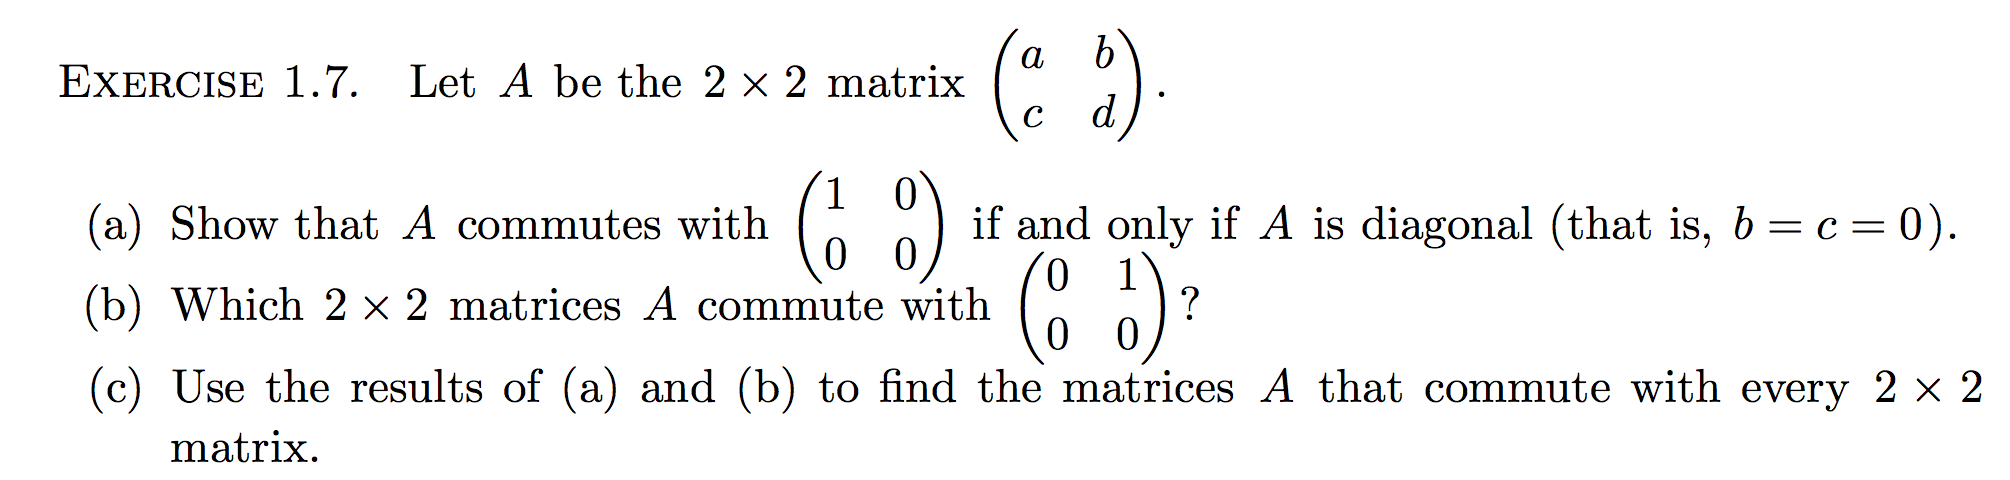
\includegraphics[width=400pt]{img/oxford-prelims-M1-linear-algebra-1-7.png}
\end{mdframed}

\begin{enumerate}[label=(\alph*)]
\item
  $\matMMxNN{a}{b}{c}{d}\matMMxNN{1}{0}{0}{0} = \matMMxNN{a}{0}
                                                         {c}{0}$.\\~\\
  $\matMMxNN{1}{0}{0}{0}\matMMxNN{a}{b}{c}{d} = \matMMxNN{a}{b}
                                                         {0}{0}$.\\~\\
  Equality iff $b = c = 0$.  I.e. matrices of the form
  $\matMMxNN{a}{0}
            {0}{d}$ (diagonal).
\item
  $\matMMxNN{a}{b}
            {c}{d}\matMMxNN{0}{1}
                           {0}{0} = \matMMxNN{0}{a}
                                             {0}{c}$.\\~\\
  $\matMMxNN{0}{1}
            {0}{0}\matMMxNN{a}{b}
                           {c}{d} = \matMMxNN{c}{d}
                                             {0}{0}$.

  Equality iff $a = d$ and $c = 0$. I.e. matrices of the form
  $\matMMxNN{a}{b}
            {0}{a}$ (upper-triangular).
\item \red{TODO}.

  Let $B = \matMMxNN{1}{0}
                    {0}{0}$. Then $B$ represents projection
  onto the first coordinate axis.

  Let $C = \matMMxNN{0}{1}
                    {0}{0}$. Then $C$ represents projection
  onto the second coordinate axis, followed by clockwise rotation through 90 degrees.

\end{enumerate}

\begin{mdframed}
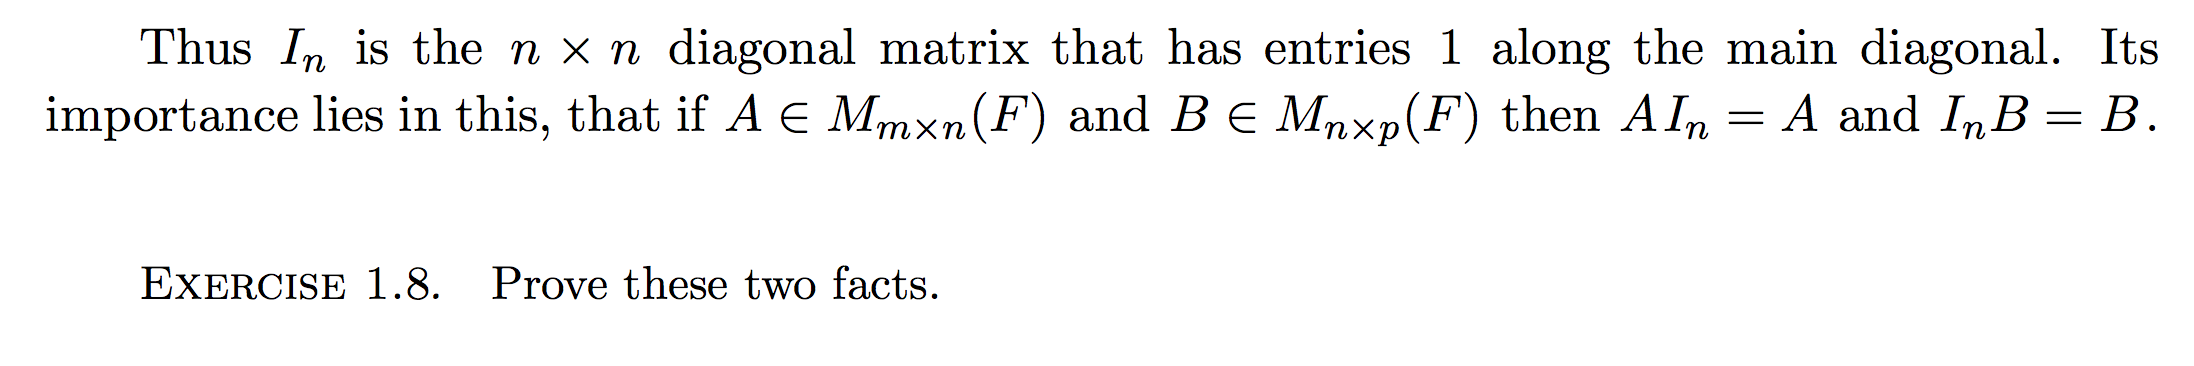
\includegraphics[width=400pt]{img/oxford-prelims-M1-linear-algebra-1-8.png}
\end{mdframed}

\begin{mdframed}
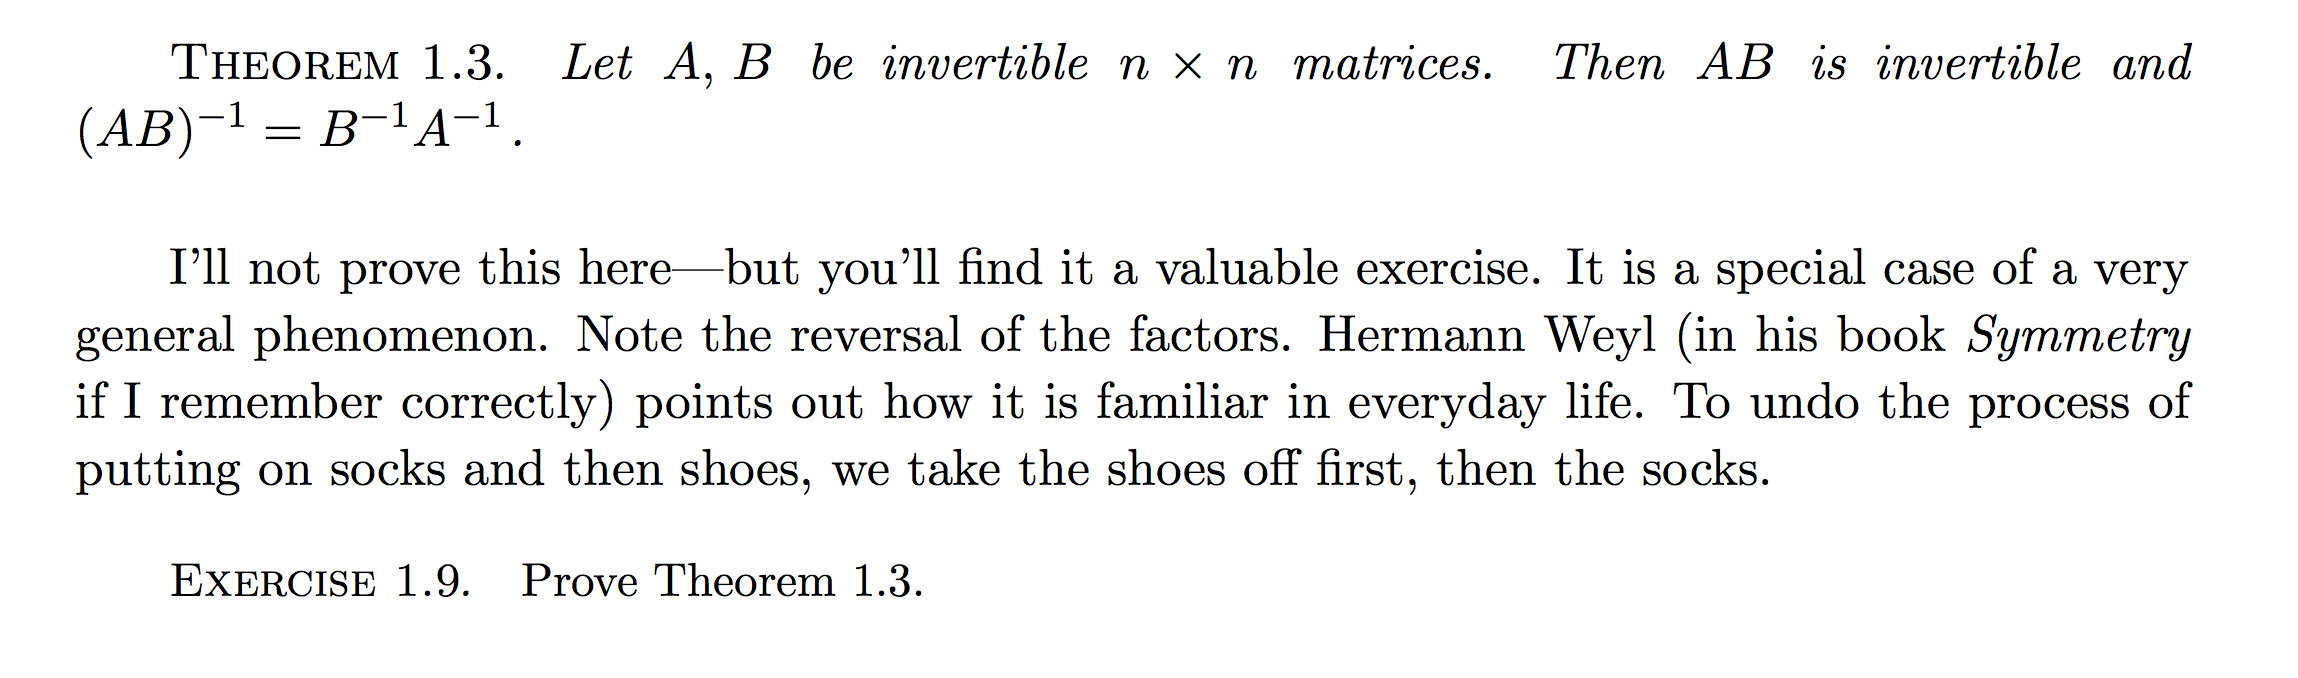
\includegraphics[width=400pt]{img/oxford-prelims-M1-linear-algebra-1-9.png}
\end{mdframed}

\begin{mdframed}
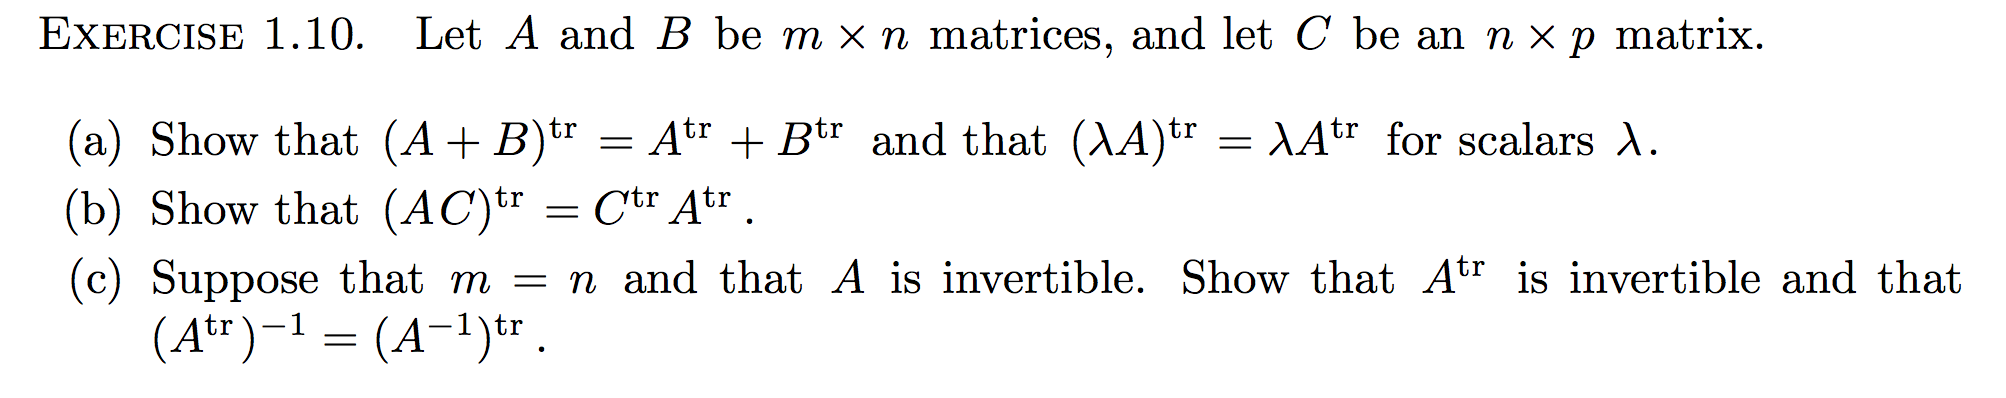
\includegraphics[width=400pt]{img/oxford-prelims-M1-linear-algebra-1-10.png}
\end{mdframed}

\begin{mdframed}
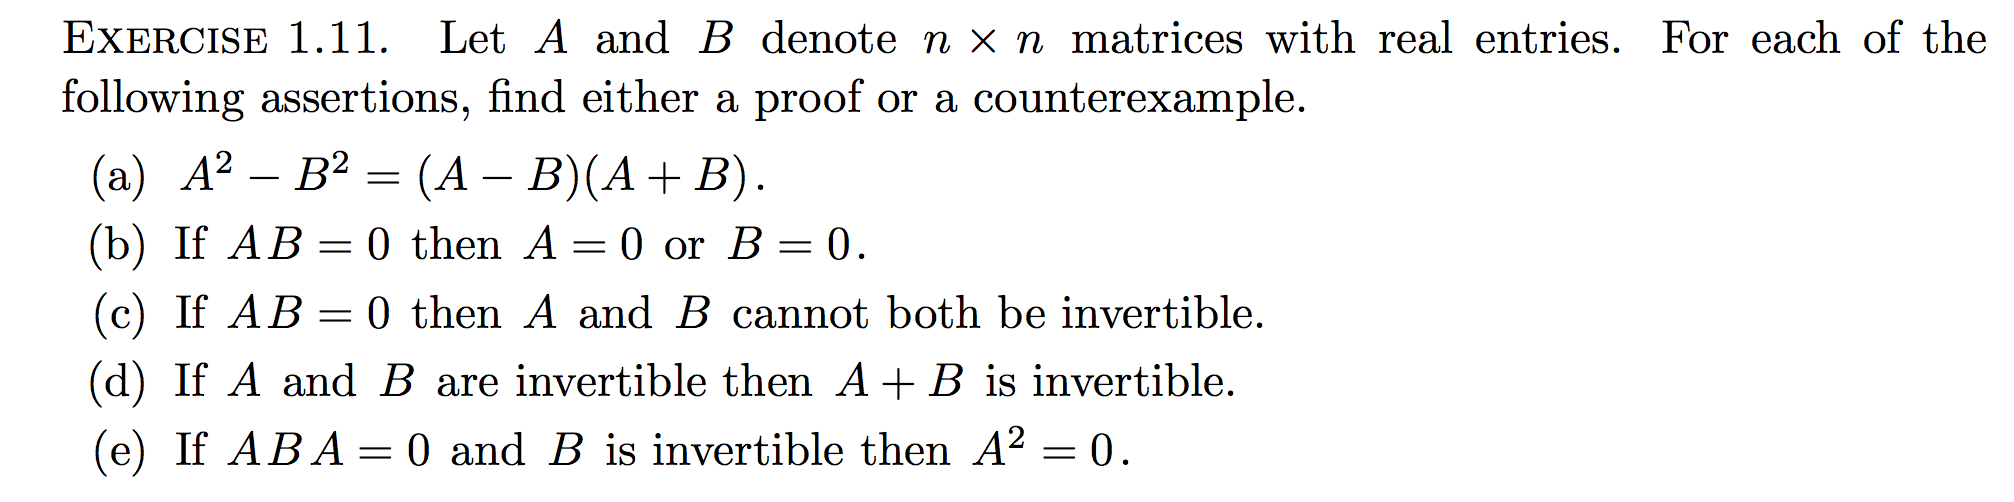
\includegraphics[width=400pt]{img/oxford-prelims-M1-linear-algebra-1-11.png}
\end{mdframed}

\begin{mdframed}
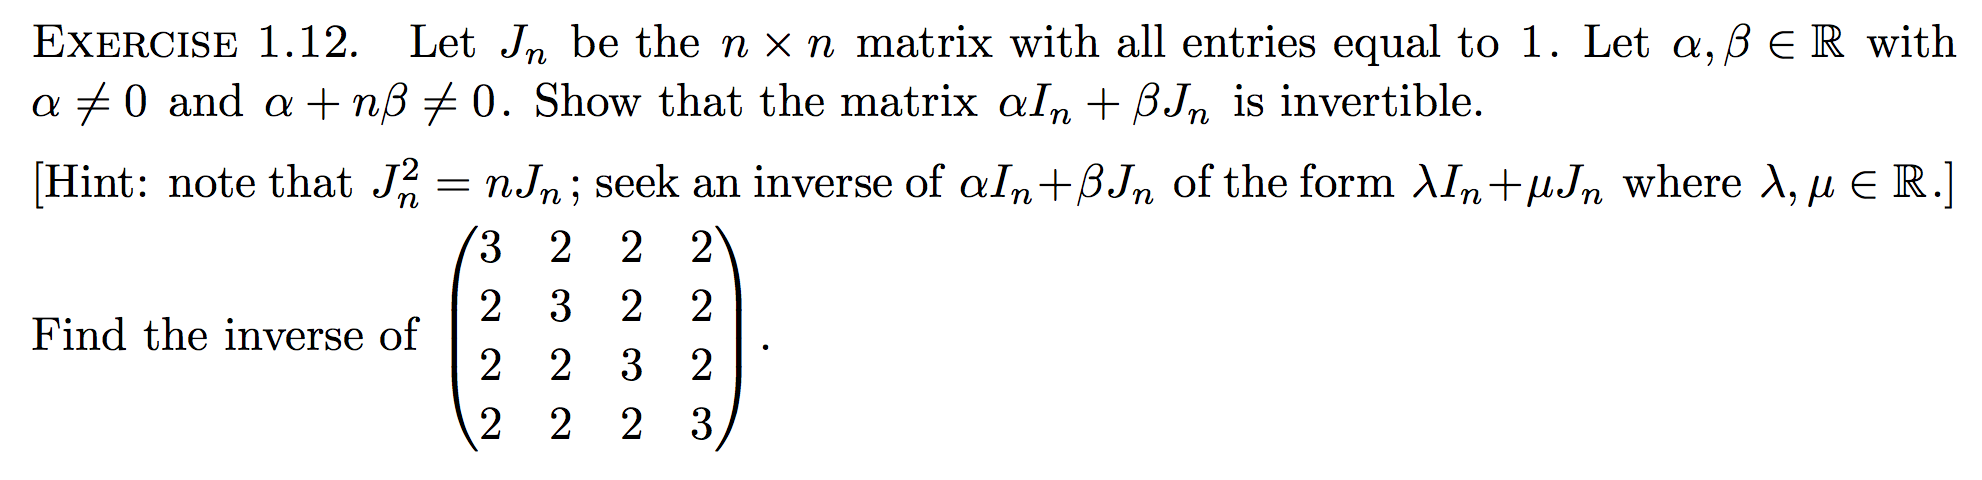
\includegraphics[width=400pt]{img/oxford-prelims-M1-linear-algebra-1-12.png}
\end{mdframed}

\begin{mdframed}
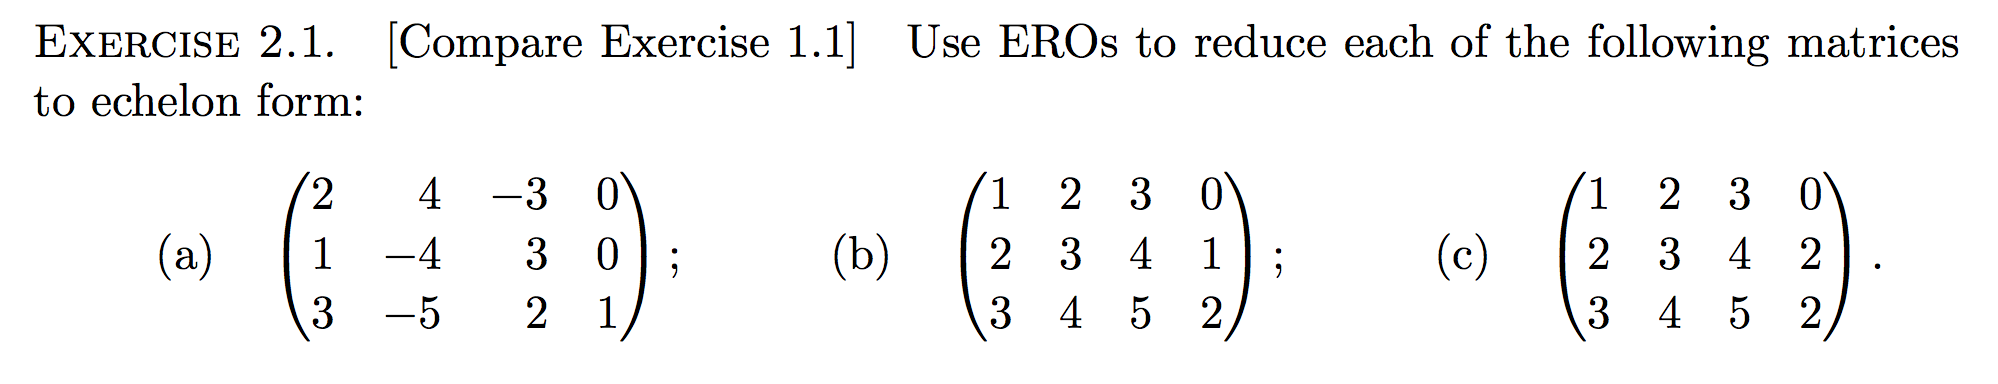
\includegraphics[width=400pt]{img/oxford-prelims-M1-linear-algebra-2-1.png}
\end{mdframed}

\begin{mdframed}
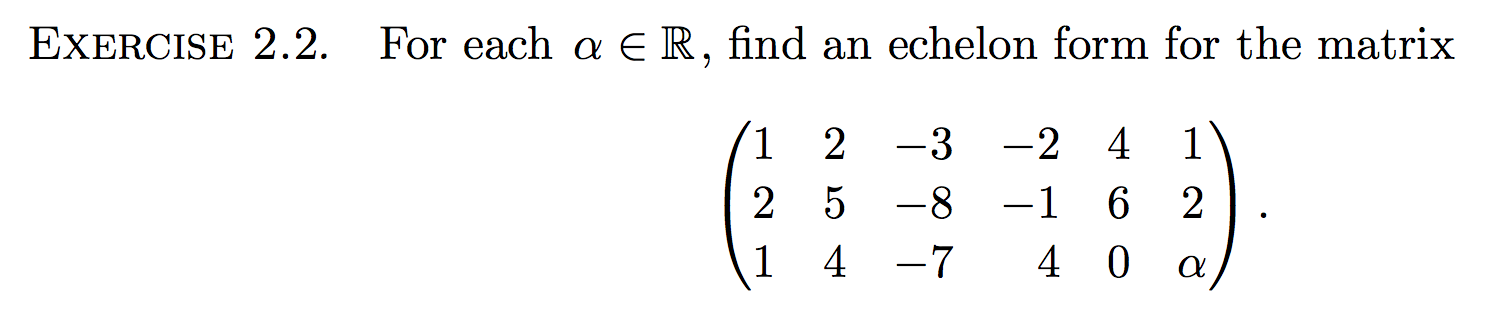
\includegraphics[width=400pt]{img/oxford-prelims-M1-linear-algebra-2-2.png}
\end{mdframed}

\begin{mdframed}
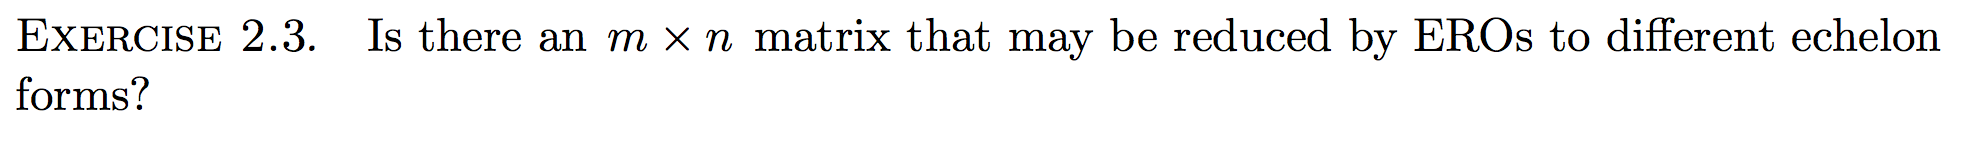
\includegraphics[width=400pt]{img/oxford-prelims-M1-linear-algebra-2-3.png}
\end{mdframed}

\begin{mdframed}
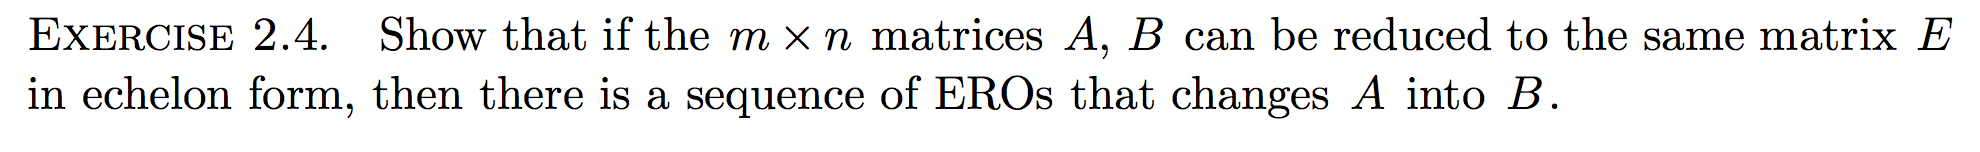
\includegraphics[width=400pt]{img/oxford-prelims-M1-linear-algebra-2-4.png}
\end{mdframed}

\begin{mdframed}
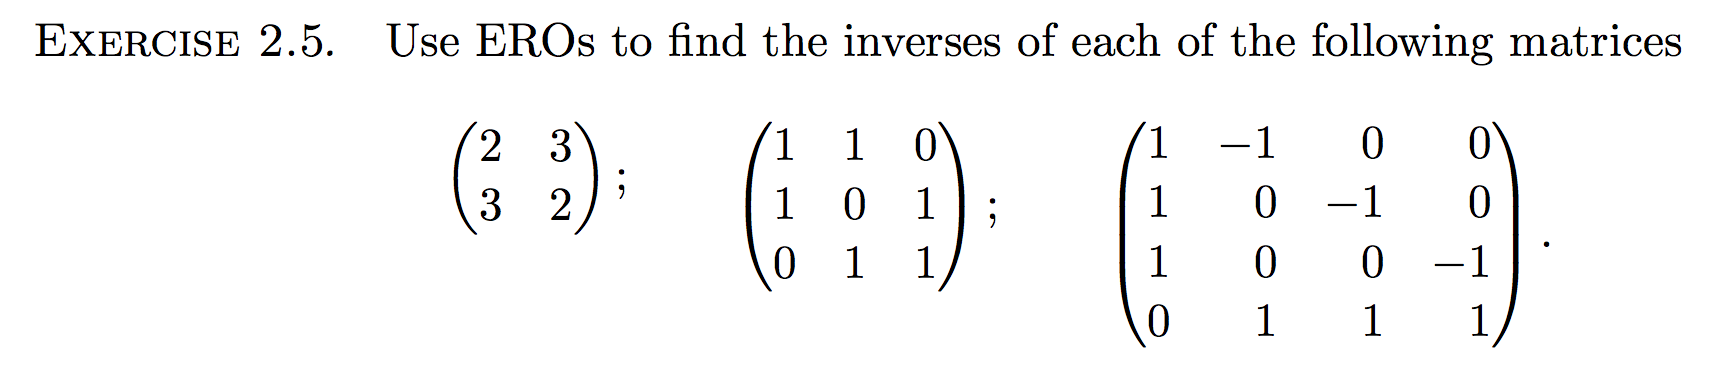
\includegraphics[width=400pt]{img/oxford-prelims-M1-linear-algebra-2-5.png}
\end{mdframed}

\begin{mdframed}
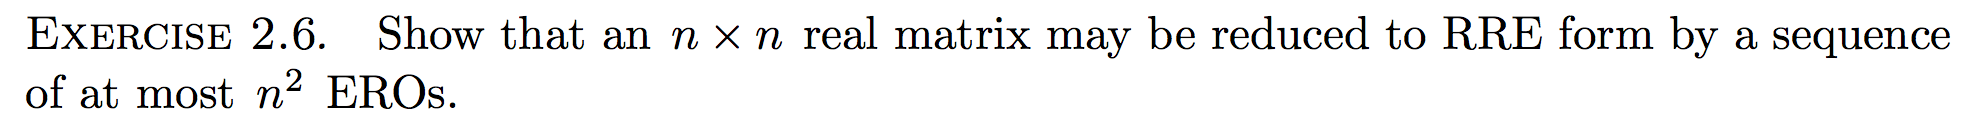
\includegraphics[width=400pt]{img/oxford-prelims-M1-linear-algebra-2-6.png}
\end{mdframed}


\newpage
\begin{mdframed}
  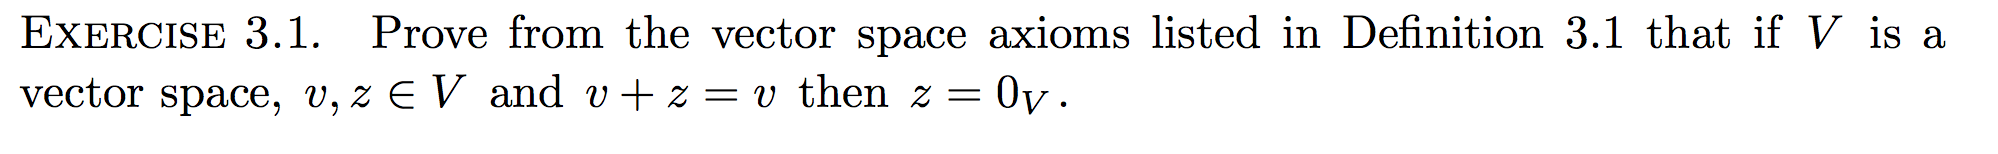
\includegraphics[width=400pt]{img/oxford-prelims-M1-linear-algebra-3-1.png}
\end{mdframed}

\begin{proof}
  From (VS4), $-z$ exists, and we have $v + z + (-z) = v = v + (-z)$, which is a
  contradiction if $z \neq 0_V$.
\end{proof}

\begin{mdframed}
  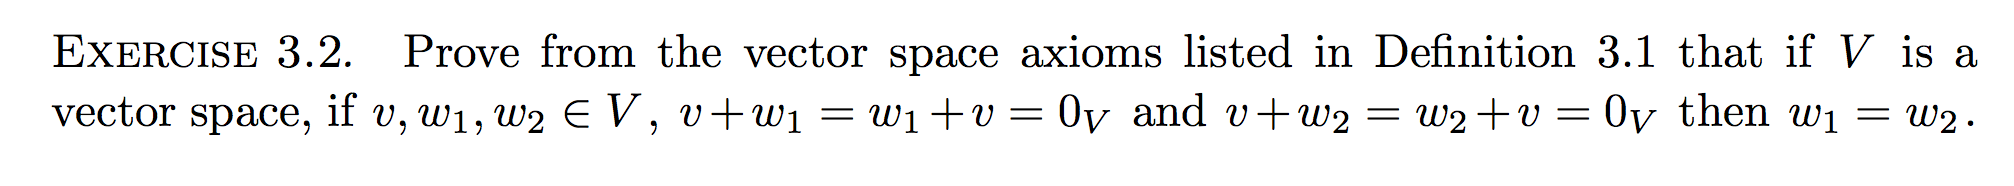
\includegraphics[width=400pt]{img/oxford-prelims-M1-linear-algebra-3-2.png}
\end{mdframed}

\begin{mdframed}
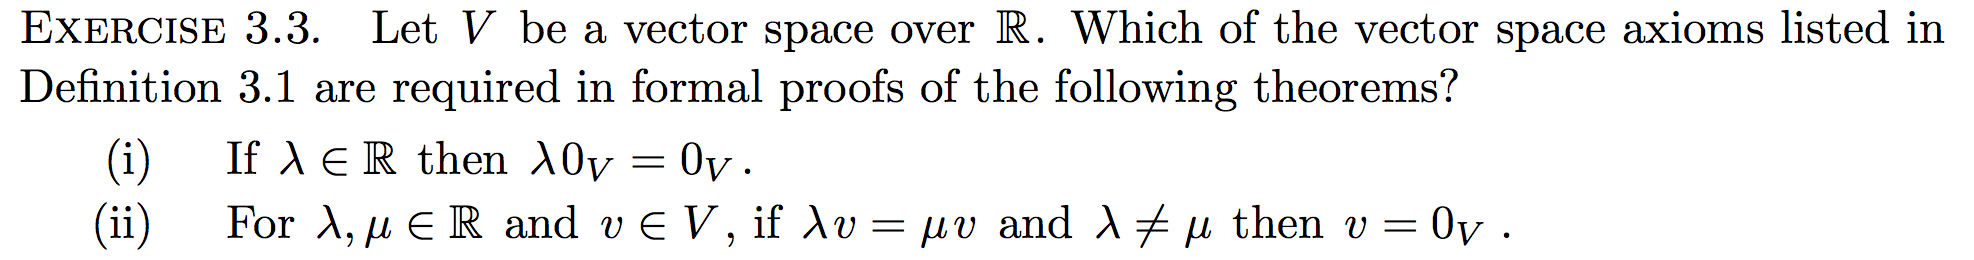
\includegraphics[width=400pt]{img/oxford-prelims-M1-linear-algebra-3-3.png}
\end{mdframed}

\begin{mdframed}
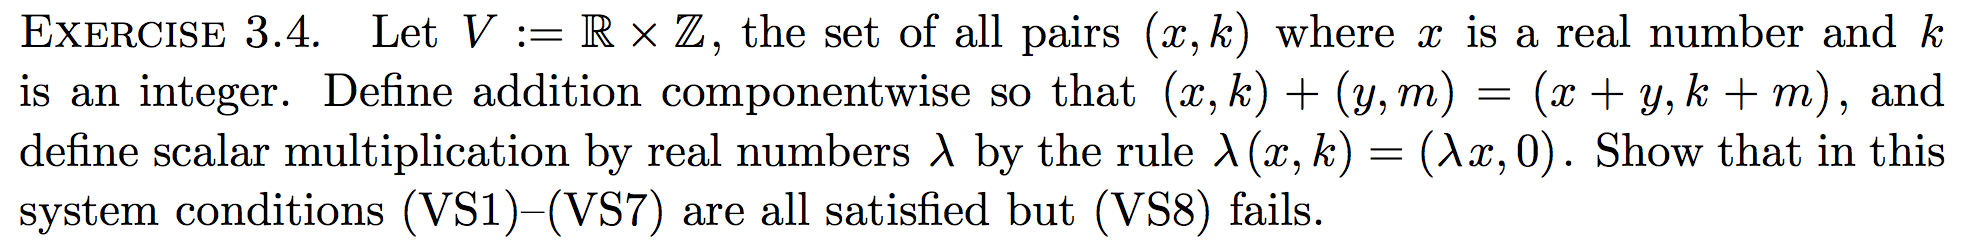
\includegraphics[width=400pt]{img/oxford-prelims-M1-linear-algebra-3-4.png}
\end{mdframed}

\begin{mdframed}
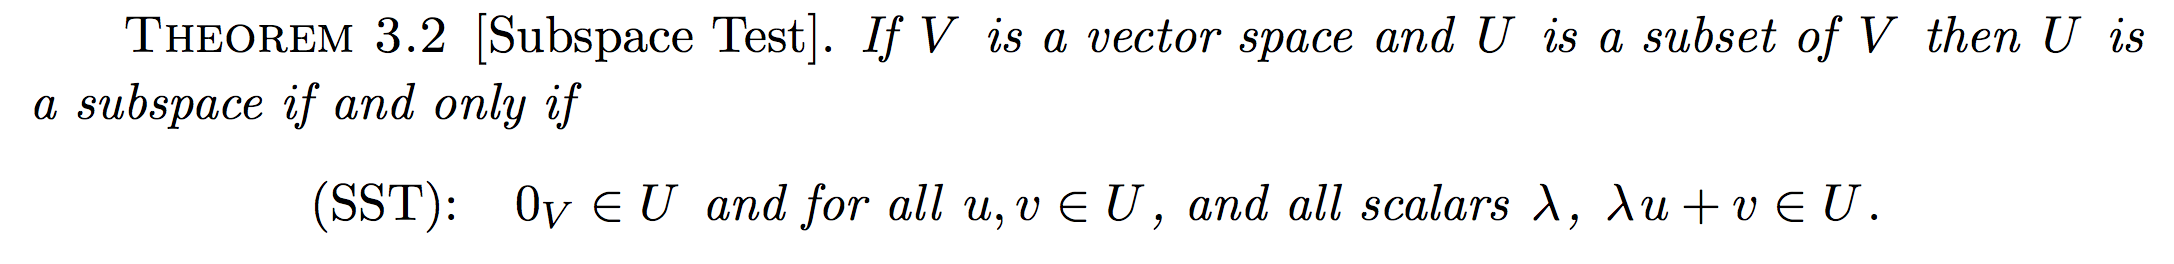
\includegraphics[width=400pt]{img/oxford-prelims-M1-linear-algebra-thm-3-2.png}
\end{mdframed}

\begin{proof}
  Suppose $U$ is a subspace of $V$. Then by definition of subspace
  (non-emptiness) $U$ is non-empty, hence $u \in U$ exists. Also by definition
  of subspace (closure under scalar multiplication) $\lambda u \in U$. In
  particular, $0u = 0_V \in U$. Finally by definition of subspace (closure
  under vector addition) $\lambda u + v \in U$, for all $u, v \in U$.

  Conversely, suppose $0_V \in U$ and $\lambda u + v \in U$ for all
  $u, v \in U$. Then $U \neq \emptyset$. Letting $\lambda = 1$ we see that
  $u + v \in U$ for all $u, v \in U$, and letting $v = 0$, we see that
  $\lambda u \in U$ for all $u \in U$.
\end{proof}

\begin{mdframed}
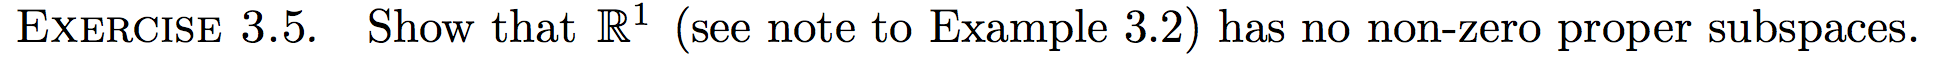
\includegraphics[width=400pt]{img/oxford-prelims-M1-linear-algebra-3-5.png}
\end{mdframed}

\begin{proof}
  Suppose $U$ is a non-zero proper subspace of $\R^1$. Then
  $\exists ~ u \in U$, and $\lambda u \in U$ for all $\lambda \in \R$, hence
  $U = \R$.
\end{proof}

\begin{mdframed}
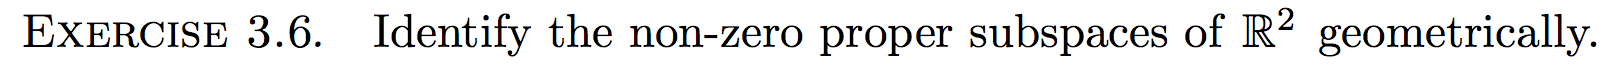
\includegraphics[width=350pt]{img/oxford-prelims-M1-linear-algebra-3-6.png}
\end{mdframed}
Take a circle with centre $(0, 0)$ and radius $r > 0$. For a point $v$ on the
circle, construct the line passing through $v$ and the origin. The set of
non-zero proper subspaces of $\R^2$ is the set of such lines.

\begin{mdframed}
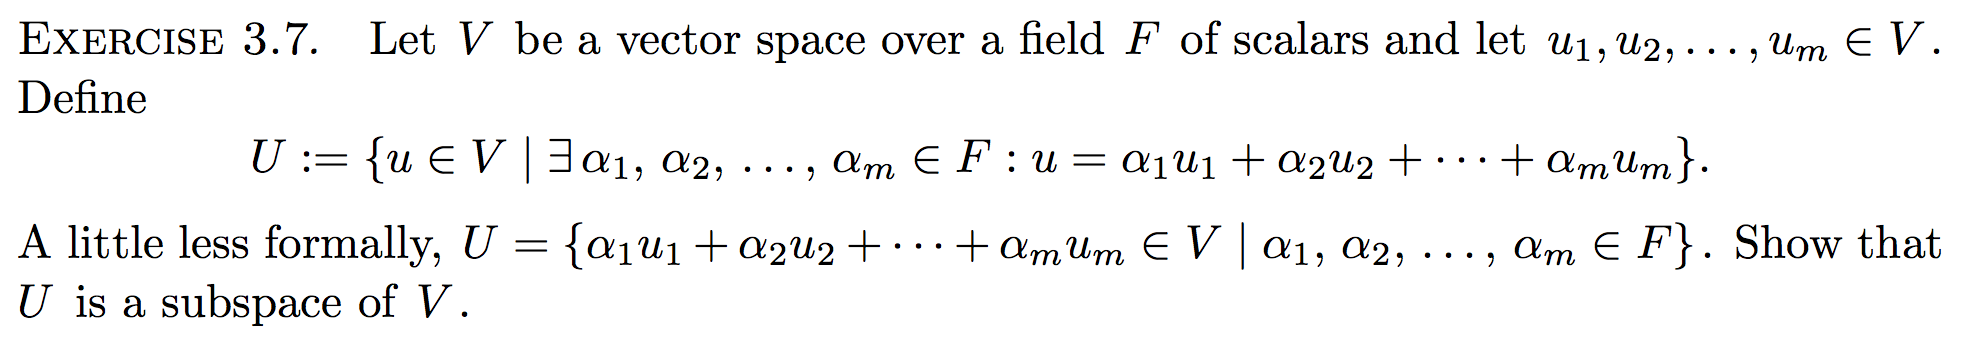
\includegraphics[width=400pt]{img/oxford-prelims-M1-linear-algebra-3-7.png}
\end{mdframed}

\begin{proof}
  $0 \in U$ since we can take all $\alpha_i = 0$.

  Let $u_1, u_2 \in U$. Then $\alpha_1u_1 + u_2 \in U$ for all $\alpha_1 \in F$
  by definition of $U$, since $\alpha_1u_1 + u_2 = \alpha_1 u_1 + \alpha_2 u_2$
  with $\alpha_2 = 1$.

  (This works even if $m = 1$ since then $u_1 = u_2$ and
  $\alpha_1u_1 + u_2 = \alpha_1 u_1 + u_1 = (\alpha_1 + 1)u_1 \in U$).
\end{proof}

\begin{mdframed}
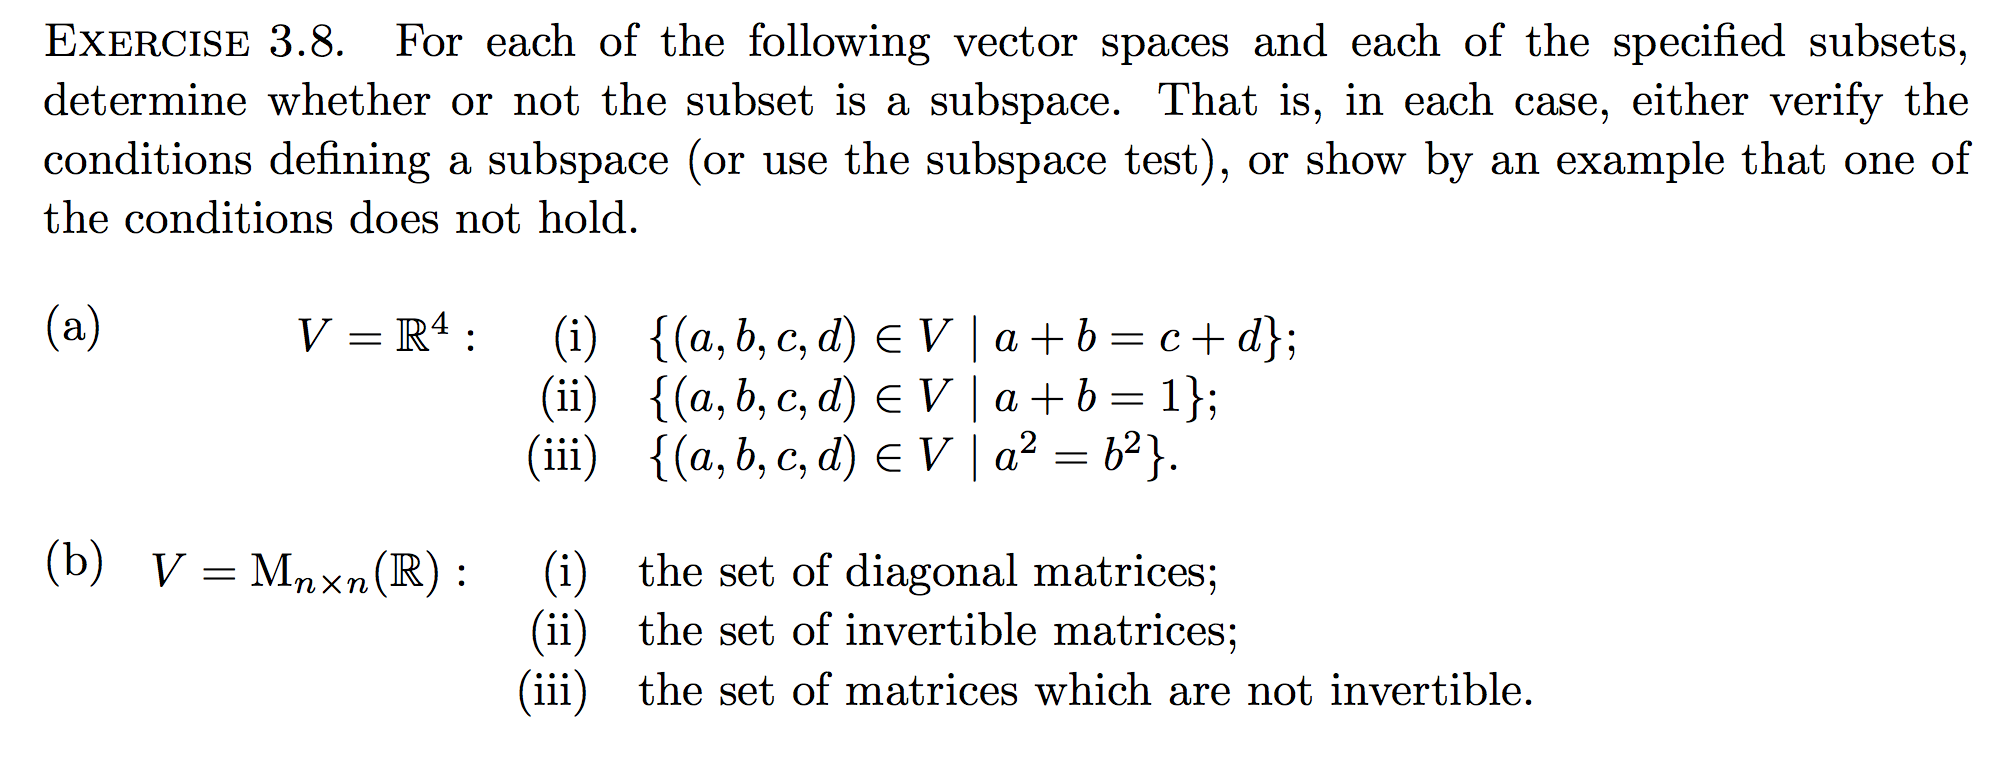
\includegraphics[width=400pt]{img/oxford-prelims-M1-linear-algebra-3-8.png}
\end{mdframed}

\begin{enumerate}[label=(\alph*)]
\item
  \begin{enumerate}[label=(\roman*)]
  \item Yes. Contains $0$ and
    \begin{align*}
      &a_1 + \lambda a_2 + b_1 + \lambda b_2 - c_1 - \lambda c_2 - d_1 - \lambda d_2\\
      =~&(a_1 + b_1) - (c_1 + d_1) + \lambda\Big((a_2 + b_2) - (c_2 + d_2)\Big)\\
      =~&0.
    \end{align*}
  \item No. Does not contain 0.
  \item No. Contains 0 but $(a_1)^2 - (b_1)^2 = (a_2)^2 - (b_2)^2 = 0 \nimplies (a_1 + a_2)^2 - (b_1 + b_2)^2 = 0$
  \end{enumerate}
\item
  \begin{enumerate}[label=(\roman*)]
  \item Yes. Contains 0 and closed under addition and scalar multiplication.
  \item No. Zero matrix not invertible.
  \item No. Neither $\matMMxNN{1}{1}
                                {1}{1}$ nor $\matMMxNN{0}{0}
                                                 {1}{2}$ are invertible.
        Yet their sum $\matMMxNN{1}{1}
                           {2}{3}$ is invertible.
  \end{enumerate}
\end{enumerate}

\begin{mdframed}
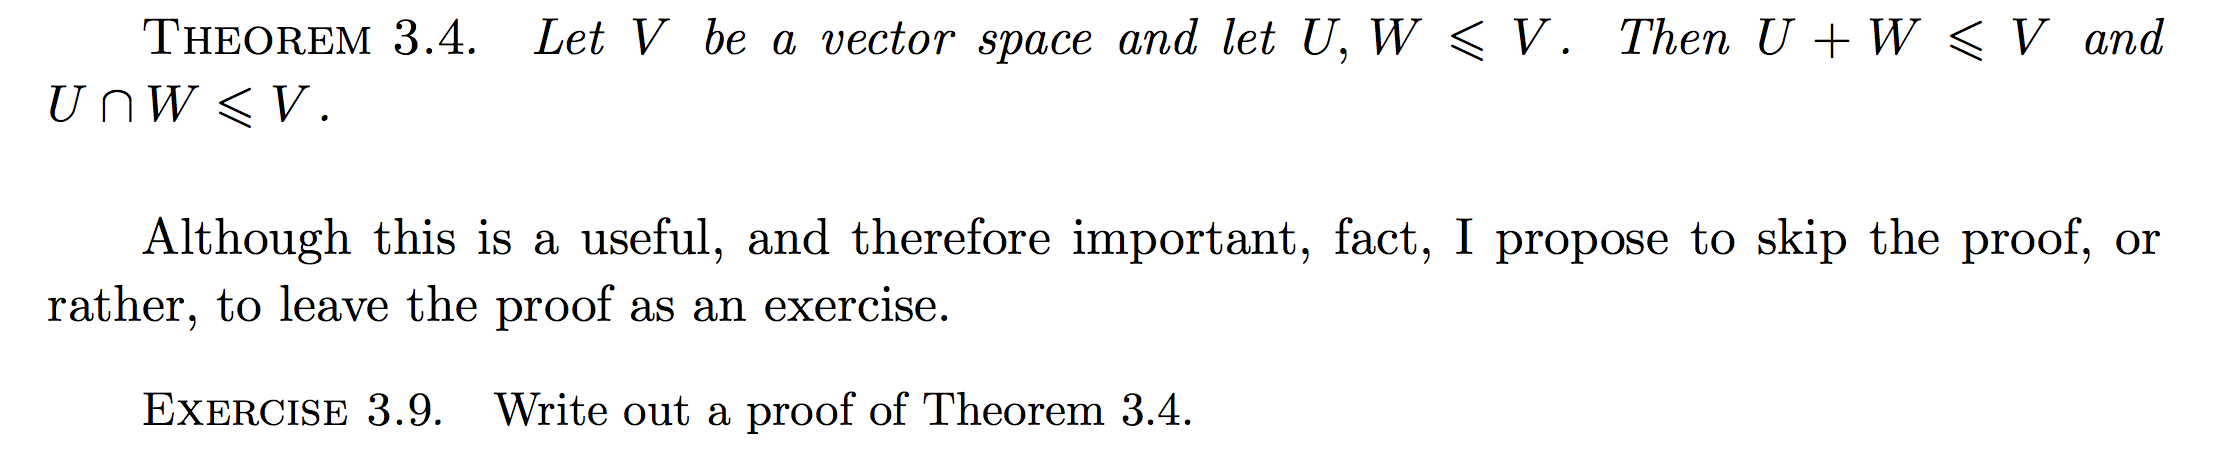
\includegraphics[width=400pt]{img/oxford-prelims-M1-linear-algebra-3-9.png}
\end{mdframed}

\begin{proof}
  $0 \in U + W$ since $0 \in U$ and $0 \in W$.

  Let $a \in U + W$. Then $a = u + w$ for some $u \in U, w \in W$. Therefore
  $a = u + w$ for some $u, w \in V$, so $a \in V$. Therefore
  $U + W \subseteq V$.

  Let $u_1, u_2 \in U$ and $w_1, w_2 \in W$, so that
  $(u_1 + w_1), (u_2 + w_2) \in U + W$, and let $\lambda$ be a scalar. Note
  that
  $$
  (u_1 + w_1) + \lambda(u_2 + w_2) = (u_1 + \lambda u_2) + (w_1 + \lambda w_2) \in U + W.
  $$
  Therefore $U + W \subspaceeq V$ by the Subspace Test.

  Regarding $U \cap V$, it contains zero and is clearly a subset of $V$. Let
  $a_1, a_2 \in U \cap V$. Then $a_1, a_2 \in U$, so
  $a_1 + \lambda a_2 \in U \subseteq V$ for all scalars $\lambda$. Therefore
  $U \cap V \subspaceeq V$.
\end{proof}

\begin{mdframed}
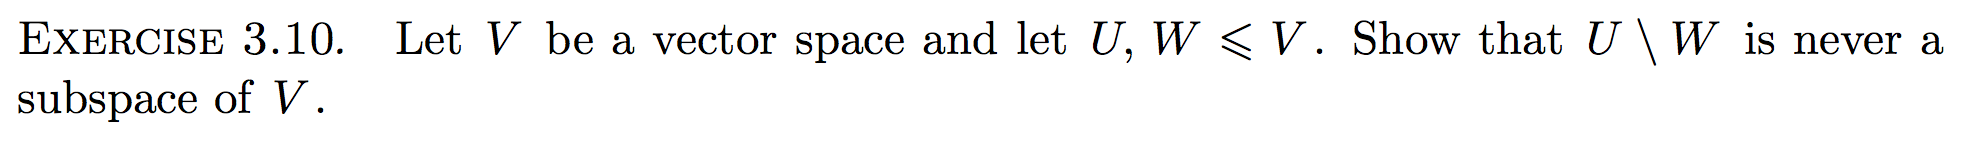
\includegraphics[width=400pt]{img/oxford-prelims-M1-linear-algebra-3-10.png}
\end{mdframed}

\begin{proof}
  $0 \notin U \setminus W$.
\end{proof}

\begin{mdframed}
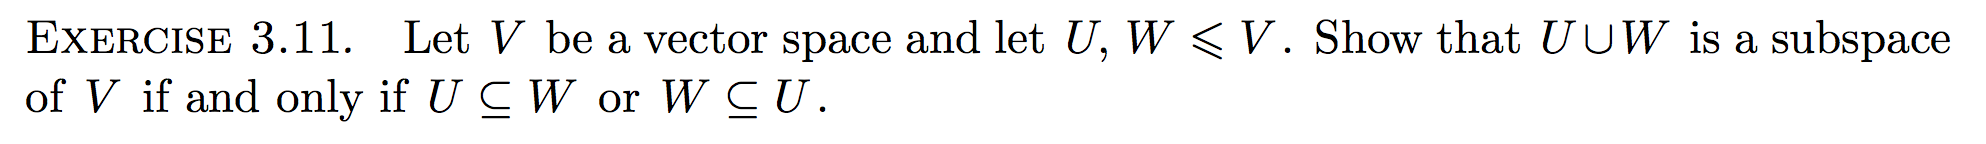
\includegraphics[width=400pt]{img/oxford-prelims-M1-linear-algebra-3-11.png}
\end{mdframed}


\begin{proof}
  First we prove that $(U \not\subseteq W$ and
  $W \not\subseteq U) \implies (U \cup V) \not\subspaceeq V$.

  Suppose that $U \not\subseteq W$ and $W \not\subseteq U$. Then there exists
  $u \in U$, $w \in W$ such that $u \notin W$ and $w \notin U$.

  Suppose $(u + w) \in U$. Then $(u + w) - u \in U$. But then $w \in U$ which
  is a contradiction. Therefore $(u + w) \notin U$.

  Similarly, $(u + w) \notin W$. Therefore $(u + w) \notin U \cup W$, and so
  $U \cup W$ is not a subspace of $V$.

  Conversely, suppose $U \subseteq W$ or $W \subseteq U$. Suppose, without loss
  of generality, that $U \subseteq W$. Then $U \cup W = W \subspaceeq V$.

  % Conversely, suppose that $U \cup W$ is not a subspace of $V$. It contains $0$
  % and is a subset, so it must fail on closure under vector addition or scalar
  % multiplication. Therefore there exists scalar $\lambda$ and
  % $v_1, v_2 \in U \cup W$ such that $v_1 + \lambda v_2 \notin U \cup W$. But
  % $v_1$ and $v_2$ cannot both be in $U$, since $U$ is a subspace, and for the
  % same reason they cannot both be in $V$. Therefore one of $v_1, v_2$ is in
  % $U \setminus W$ and the other is in $W \setminus U$. Therefore
  % $U \not\subseteq W \land W \not\subseteq U$.
\end{proof}

\begin{mdframed}
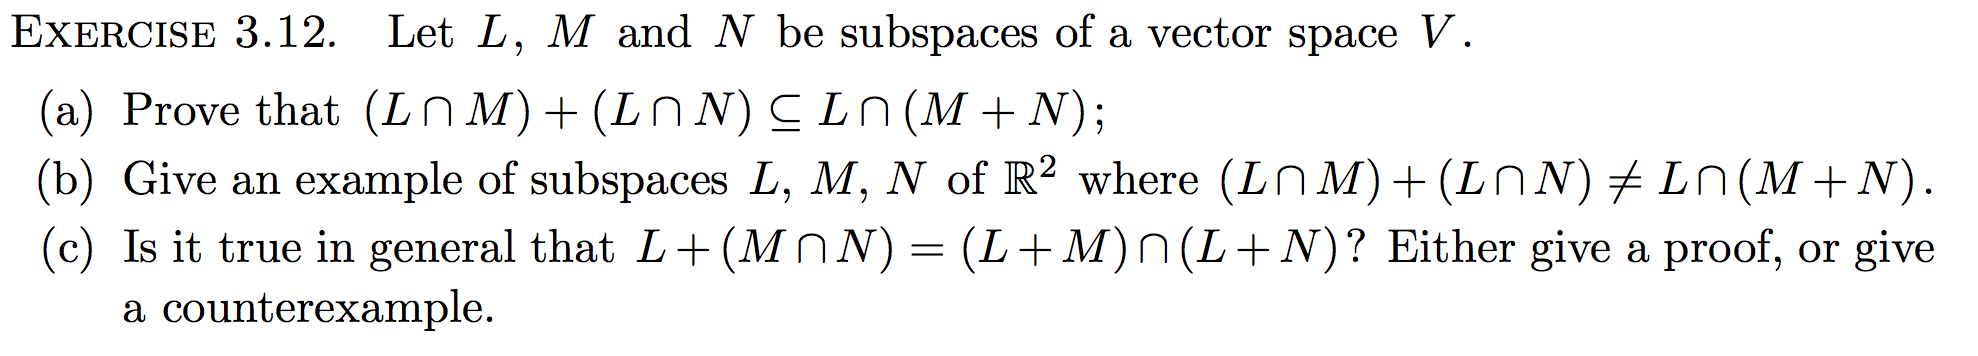
\includegraphics[width=400pt]{img/oxford-prelims-M1-linear-algebra-3-12.png}
\end{mdframed}

\begin{enumerate}[label=(\alph*)]
\item Let $v_1 \in (L \cap M) + (L \cap N)$. Then $v_1 = v_2 + v_3$ where
  $v_2, v_3 \in L$. Therefore $v_1 \in L$ since $L$ is a subspace. Also
  $v_2 \in M$ and $v_3 \in N$, therefore $v_1 \in M + N$. Therefore
  $v_1 \in L \cap (M + N)$.

\item Suppose $L =$ (line through $(1, 0)$), $M =$ (line through $(1,1)$) and
  $N = $ (line through $(0, 1)$). Then $(L \cap M) + (L \cap N) = \{0\}$. But
  $(M + N) = \R^2$, so $L \cap (M + N) = L \neq \{0\}$.

\item No, it's not true in general. Let $L, M, N$ be the lines in $\R^2$
  defined in (b) above. Then $L + (M \cap N) = L$. But
  $(L + M) \cap (L + N) = \R^2 \cap \R^2 = \R^2 \neq L$.
\end{enumerate}

\begin{mdframed}
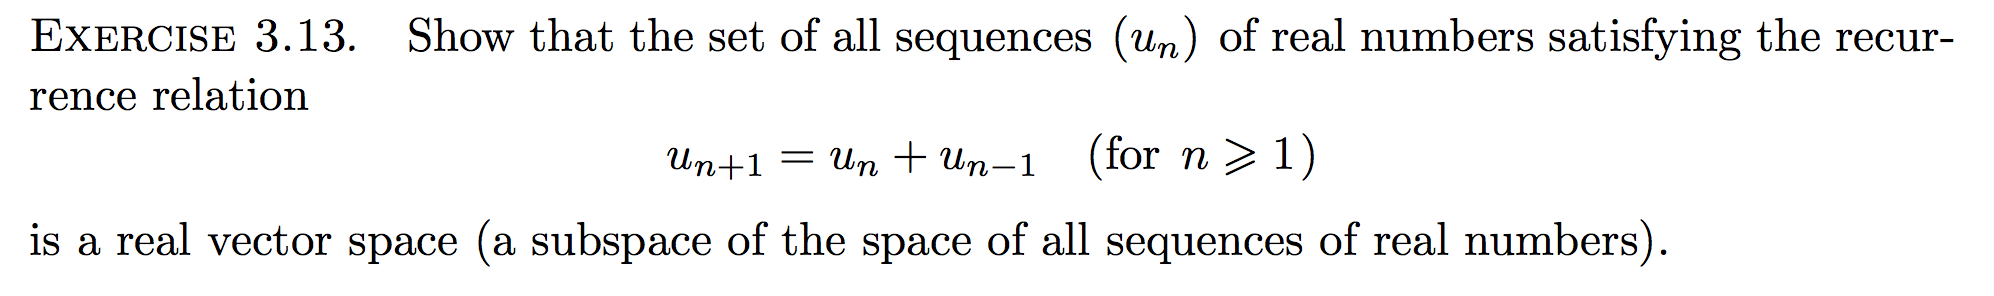
\includegraphics[width=400pt]{img/oxford-prelims-M1-linear-algebra-3-13.png}
\end{mdframed}

\begin{proof}
  Let $U$ be the set of all sequences described. Then $U$ contains the zero
  sequence $(0, 0, \ldots)$. Let $(u_n) \in U$ and $(v_n) \in U$ and let
  $(w_n) = (u_n) + \lambda(v_n)$. Then
  \begin{align*}
    w_{n+1} &= u_{n+1} + \lambda v_{n+1}\\
            &= (u_n + u_{n-1}) + \lambda (v_n + v_{n-1})\\
            &= (u_n + \lambda v_n) + (u_{n-1} + \lambda v_{n-1})\\
            &= w_n + w_{n-1}.
  \end{align*}
  So $(w_n) \in U$. Therefore $U$ is a subspace by the subspace test.
\end{proof}

\begin{mdframed}
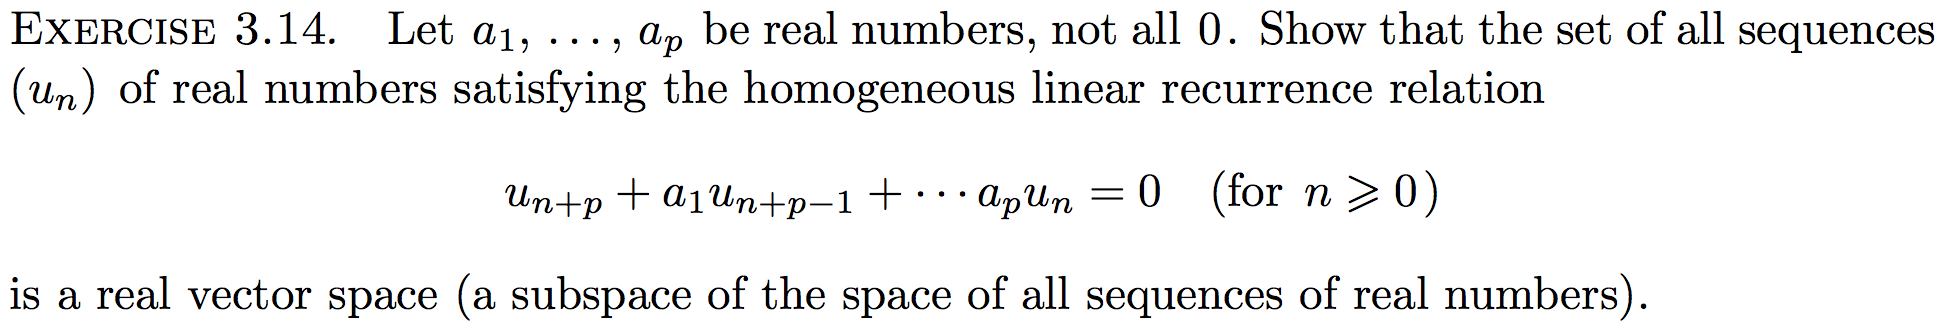
\includegraphics[width=400pt]{img/oxford-prelims-M1-linear-algebra-3-14.png}
\end{mdframed}

\begin{proof}
  Let $U$ be the set of all sequences described. Then $U$ contains the zero
  sequence $(0, 0, \ldots)$. Let $(u_n) \in U$ and $(v_n) \in U$ and let
  $(w_n) = (u_n) + \lambda(v_n)$. Then
  \begin{align*}
    % w_{n+p} + \alpha_1w_{n + p - 1} + \cdots + \alpha_pw_n
    % &=
        w_{n+p}                    + \sum_{i=1}^{p} \alpha_i w_{n+p-i}
    &= (u_{n+p} + \lambda v_{n+p}) + \sum_{i=1}^{p} \alpha_i (u_{n+p-i} + \lambda v_{n+p-i})\\
      &= (u_{n+p} + \sum_{i=1}^{p} \alpha_i u_{n+p-i}) +
        \lambda (v_{n+p} + \sum_{i=1}^{p} \alpha_i v_{n+p-i})\\
      &= 0 + \lambda \cdot 0 = 0.
  \end{align*}
  So $(w_n) \in U$. Therefore $U$ is a subspace by the subspace test.
\end{proof}

\begin{mdframed}
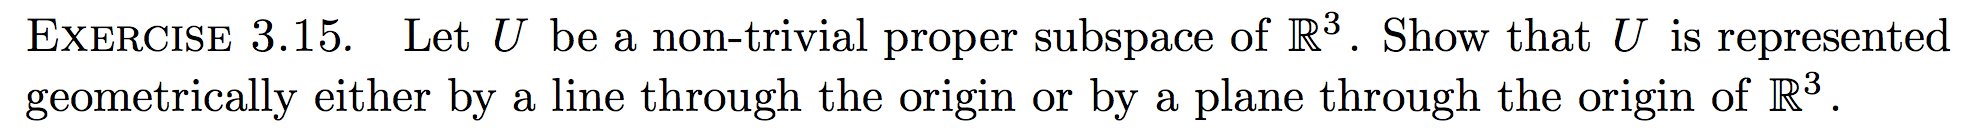
\includegraphics[width=400pt]{img/oxford-prelims-M1-linear-algebra-3-15.png}
\end{mdframed}

\begin{proof}

\end{proof}


\section{2017}

\subsection*{}  % 1
\begin{mdframed}
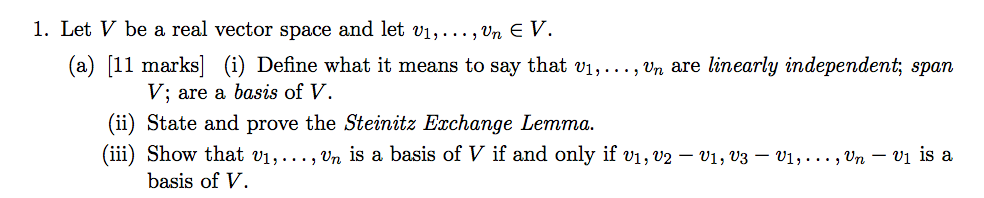
\includegraphics[width=400pt]{img/oxford-prelims-2017-A-1-1.png}
\end{mdframed}

\subsubsection*{(i)}
\begin{definition*}[Linear independence]
  Let $a_1, \ldots, a_n \in \R$. Then $v_1, v_2, \ldots, v_n$ are linearly
  independent if and only if the only solution to $\sum_{i=1}^n a_iv_i = 0$ is
  $a_1 = a_2 = \ldots = a_n = 0$.
\end{definition*}

\begin{definition*}[Span]
  $v_1, v_2, \ldots, v_n$ span $V$ if and only if for all $w \in V$ there exist
  $a_1, \ldots, a_n \in \R$ such that $\sum_{i=1}^n a_iv_i = w$.
\end{definition*}

\begin{definition*}[Basis]
  $v_1, v_2, \ldots, v_n$ are a basis for $V$ if and only if they span $V$ and
  they are linearly independent.
\end{definition*}

\subsubsection*{}
\begin{mdframed}
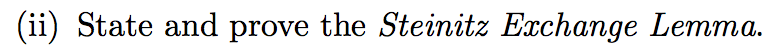
\includegraphics[width=250pt]{img/oxford-prelims-2017-A-1-1-2.png}
\end{mdframed}

\newpage
\begin{theorem*}[Steinitz Exchange Lemma - version 1]
  Let $X$ be a subset of a vector space $V$. Let $u \in \Span X$. Let $v \in X$
  be such that $u \notin \Span\(X \setminus \{v\}\)$. Then
  $\Span\(\(X \setminus \{v\}\) \cup \{u\}\) = \Span X$.
\end{theorem*}

[Informally: Take a set of vectors, one of which is $v$. Suppose their span
contains $u$, but, after removing $v$, their span no longer contains $u$. Now
consider the set resulting after exchanging $u$ for $v$. The span of this set
is the same as that of the original.]

\begin{proof}~\\
  Let $X$ be $\{v_1, \ldots, v_n\}$, and let $u \in \Span X$.

  Reorder the $v_i$ such that $u \notin \Span\(v_2, \ldots, v_n\)$.

  Note that $u = \sum_{i=1}^n\gamma_iv_i$ for some
  $\gamma_1, \ldots, \gamma_n \in \R$, where $\gamma_1 \neq 0$.

  Therefore $v_1 = \frac{1}{\gamma_1}\(u - \sum_{i=2}^n\gamma_iv_i\)$.

  So we have $u \in \Span\(v_1, \ldots, v_n\)$ and
  $v_1 \in \Span\(u, v_2, \ldots, v_n\)$.

  It is clear\footnote{
    For the forwards direction, let $w$ be in $\Span\(u, v_2, \ldots,
    v_n\)$. We have $w = au + \sum_{i=2}^n\lambda_iv_i$ for some
    $a, \lambda_2, \ldots, \lambda_n \in \R$, and therefore
    $$
      w = a\sum_{i=1}^n\gamma_iv_i + \sum_{i=2}^n\lambda_iv_i
        = a\gamma_1v_1 + \sum_{i=2}^n(\gamma_i + \lambda_i)v_i,
    $$
    proving that $w \in \Span\(v_1, \ldots, v_n\)$, as required. For the
    reverse direction, let $w$ be in $\Span~ \{v_1, \ldots, v_n\}$. We have
    $w = \sum_{i=1}^n\lambda_iv_i$ for some
    $a, \lambda_2, \ldots, \lambda_n \in \R$, and therefore
    $$
      w = \frac{\lambda_1}{\gamma_1}\(u - \sum_{i=2}^n\gamma_iv_i\) + \sum_{i=2}^n\lambda_iv_i
        = \frac{\lambda_1}{\gamma_1}u + \sum_{i=2}^n(\lambda_i - \gamma_i)v_i,
    $$
    proving that $w \in \Span\(u, v_2, \ldots, v_n\)$, as required.  } that any
  vector in $\Span\(u, v_2, \ldots, v_n\)$ can be rewritten as a linear
  combination of $v_1, \ldots, v_n$, and conversely that any vector in
  $\Span\(v_1, \ldots, v_n\)$ can be rewritten as a linear combination of
  $u, v_2, \ldots, v_n$.

\end{proof}

\newpage
\begin{theorem*}
  A linearly independent set can be no larger than a spanning set.
\end{theorem*}

\begin{proof}
  Let $V$ be a vector space.

  Let $S = u_1, \ldots, u_m$ be linearly independent vectors in $V$.

  Let $T = v_1, \ldots, v_n$ span $V$.

  The argument involves repeatedly substituting members of the two sets so that
  after $m$ steps, $m$ members of $T$ have been removed, each time being
  replaced by a member of $S$.

  Therefore $m \leq n$, i.e. a linearly independent set can be no larger than a
  spanning set.

\end{proof}

\begin{theorem*}
  Every basis has the same size.
\end{theorem*}

\begin{theorem*}
  A spanning set that is the same size as a basis is also a basis.
\end{theorem*}



\newpage
\subsubsection*{}
\begin{mdframed}
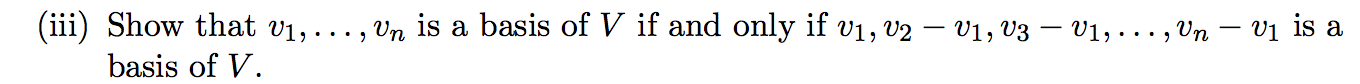
\includegraphics[width=400pt]{img/oxford-prelims-2017-A-1-1-3.png}
\end{mdframed}


\begin{proof}~\\
$\implies$\\
For the forward implication, suppose that $v_1, \ldots, v_n$ is a basis of $V$.

Then for all $w \in V$ there exist unique coordinates $\lambda_1, \ldots, \lambda_n$ such that
\begin{align*}
  \sum_{i=1}^n \lambda_iv_i &= w.
\end{align*}
Subtracting $\(\sum_{i=1}^n \lambda_i\)v_1$ from both sides we have
\begin{align*}
  \sum_{i=1}^n \lambda_i(v_i - v_1) &= w - \(\sum_{i=1}^n \lambda_i\)v_1\\
  \(\sum_{i=1}^n \lambda_i\)v_1 + \sum_{i=2}^n \lambda_i(v_i - v_1) &= w,
\end{align*}
proving that $v_1, v_2 - v_1, \ldots, v_n - v_1$ spans $V$.

Furthermore, $v_1, v_2 - v_1, \ldots, v_n - v_1$ are linearly independent,
since a corollary of the Steinitz Exchange Lemma is that if a spanning set is
the same size as a linearly independent set, then the spanning set is also
linearly independent (and the linearly independent set spans, so in fact both
are bases).

$\impliedby$\\
For the reverse implication, suppose that $v_1, v_2 - v_1, \ldots, v_n - v_1$
is a basis of $V$.

Then for all $w \in V$ there exist unique coordinates $\lambda_1, \ldots, \lambda_n$ such that
\begin{align*}
  \lambda_1v_1 + \sum_{i=2}^n \lambda_i(v_i - v_1) = w.
\end{align*}
Equivalently,
\begin{align*}
  \Big(\lambda_1 - \sum_{i=2}^n\lambda_i\Big)v_1 + \sum_{i=2}^n \lambda_iv_i = w,
\end{align*}

proving that $v_1, v_2, \ldots, v_n$ span $V$.

Furthermore, $v_1, v_2, \ldots, v_n$ are linearly independent, by the same
Steinitz Exchange Lemma argument given above.
\end{proof}

~\\
\newpage
\begin{mdframed}
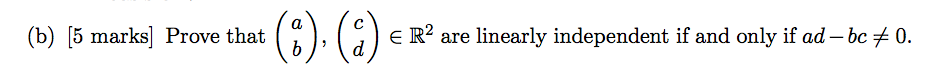
\includegraphics[width=400pt]{img/oxford-prelims-2017-A-1-2.png}
\end{mdframed}

\renewcommand{\cvec}[2]{\begin{pmatrix}#1\\#2\end{pmatrix}}

\begin{proof}
  For the forwards implication, suppose for a contradiction that $\cvec{a}{b}$
  and $\cvec{c}{d}$ are linearly independent and $ad - bc = 0$.

  Note that $d\cvec{a}{b} - b\cvec{c}{d} = \cvec{0}{0}$. But this contradicts
  linear independence, since if $b = d = 0$ then $\cvec{a}{b} = \cvec{a}{0}$
  and $\cvec{c}{d} = \cvec{c}{0}$ are linearly dependent.

  Therefore linear independence implies $ad - bc \neq 0$.

  For the reverse implication, suppose for a contradiction that $\cvec{a}{b}$
  and $\cvec{c}{d}$ are linearly dependent and $ad - bc \neq 0$.

  Note that $\cvec{c}{d} = \lambda \cvec{a}{b}$ for some $\lambda \in \R$.

  % Consider $\lambda_1\cvec{a}{b} + \lambda_2 \cvec{c}{d} = \cvec{0}{0}$.

  Therefore $d\cvec{a}{b} - b\cvec{c}{d} = d\cvec{a}{b} - b\lambda\cvec{a}{b}$,
  giving the following system of equations:
  \begin{align*}
    \begin{cases}
      ab\lambda &= bc\\
      bd        &= b^2\lambda.
    \end{cases}
  \end{align*}
  Suppose that $b \neq 0$. Then $d = b\lambda$, hence $ad = bc$, a contradiction.

  Alternatively, suppose $b = 0$. Then in order for $\cvec{a}{b} = \cvec{a}{0}$
  and $\cvec{c}{d}$ to be linearly dependent, we must have $d = 0$ (OK?). In
  which case $ad - bc = 0$, a contradiction again.

  Therefore $ad - bc \neq 0$ implies linear independence.

\end{proof}

\newpage

\begin{proof}
Let $x_1 = \cvec{a}{b}$ and $x_2 = \cvec{c}{d}$

We prove the negation; that $x_1, x_2$ linearly dependent is equivalent to
$ad - bc = 0$.

$\implies$\\
For the forwards implication, we prove that $x_1, x_2$ linearly dependent
implies $ad - bc = 0$.

Since they are linearly dependent, there exists $\lambda_1, \lambda_2 \in \R$
such that $\lambda_1x_1 + \lambda_2x_2 = 0$, with at least one of
$\lambda_1, \lambda_2$ non-zero.

Suppose, without loss of generality, that $\lambda_1 = 0$. Then
$\lambda_2 \neq 0$ and therefore $c = d = 0$, and therefore $ad - bc = 0$.

The remaining case is that $\lambda_1 \neq 0$ and $\lambda_2 \neq 0$. Then
\begin{align*}
  \begin{cases}
    a\lambda_1 + c\lambda_2 = 0\\
    b\lambda_1 + d\lambda_2 = 0,
  \end{cases}
\end{align*}
therefore
\begin{align*}
  \lambda_1                            &= -\frac{c}{a}\lambda_2\\
  \Big(-\frac{bc}{a} + d\Big)\lambda_2 &= 0\\
  ad - bc                              &= 0.
\end{align*}

$\impliedby$\\
For the reverse implication, we prove that $ad - bc = 0$ implies $x_1, x_2$
linearly dependent.

\red{TODO: Not sure how to do this without resorting to properties of
  determinant of linear transformation.}

Let $u_1, u_2$ be a basis for $\R^2$ and consider the matrix
$\matMMxNN{a}{c} {b}{d}$ with respect to this basis.

Viewed as a linear transformation, the matrix sends $u_1 \mapsto x_1$ and
$u_2 \mapsto x_2$.

The determinant of this matrix is $ad - bc$. Since the determinant is zero, the
linear transformation maps the basis vectors into a one- or zero-dimensional
subspace.

Therefore $x_1,x_2$ lie in a one dimensional subspace. Therefore
$x_1 = \lambda x_2$ for some $\lambda \in \R$. Therefore $x_1,x_2$ are linearly
dependent.

\end{proof}

\begin{mdframed}
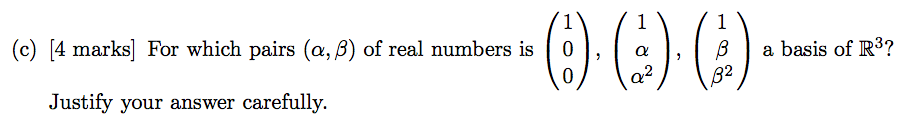
\includegraphics[width=400pt]{img/oxford-prelims-2017-A-1-3.png}
\end{mdframed}

To be a basis they must be linearly independent, and must span $\R^3$.

Since there are 3 of them, if they are linearly independent, then they span (by
Steinitz exchange lemma).

Suppose

\begin{align*}
  \begin{cases}
    \lambda_1 + \lambda_2 + \lambda_3    &= 0\\
    \lambda_2\alpha + \lambda_3\beta     &= 0\\
    \lambda_2\alpha^2 + \lambda_3\beta^2 &= 0
  \end{cases}
\end{align*}


has a solution other than $\lambda_1 = \lambda_2 = \lambda_3 = 0$. Then either
$\lambda_2 \neq 0$ or $\lambda_3 \neq 0$. Suppose that $\lambda_2 \neq 0$. Then
$\alpha = -\frac{\lambda_3}{\lambda_2}\beta$. Therefore
\begin{align*}
  \frac{\lambda_3^2}{\lambda_2}\beta^2 + \lambda_3\beta^2 &= 0\\
  \beta^2\(\frac{\lambda_3^2}{\lambda_2} + \lambda_3\) &= 0\\
\end{align*}

\red{TODO}

\subsection*{}  % 2
\begin{mdframed}
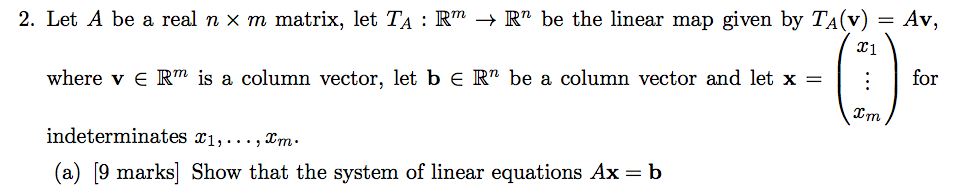
\includegraphics[width=400pt]{img/oxford-prelims-2017-A-2-1.png}
\end{mdframed}

\subsection*{}  % 2.a.i
\begin{mdframed}

\includegraphics[width=400pt]{img/oxford-prelims-2017-A-2-1-1.png}
\end{mdframed}

By definition,  $\Im T_A = \{Ax: x \in \R^m\}$.

Let $S$ denote the proposition ``$Ax = b$ has a solution''.

By the definition of ``has a solution'', $S$ is equivalent to the proposition
``there exists $x \in \R^m$ such that $Ax = b$''.

We see that $S \implies b \in \Im T_A$, and also that $b \in \Im T_A \implies S$.

\subsubsection*{} % 2.a.ii
\begin{mdframed}
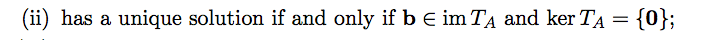
\includegraphics[width=350pt]{img/oxford-prelims-2017-A-2-1-2.png}
\end{mdframed}

Let $S_u$ denote the proposition ``$Ax = b$ has a unique solution''.

First we prove the forwards implication:

\begin{claim*}
  $S_u \implies \Big(b \in \Im T_A ~~\text{and}~~ \ker T_A = \{0\}\Big)$.
\end{claim*}

\begin{proof}
Firstly, since $S_u \implies S$, we know from part (i) that
$S_u \implies b \in \Im T_A$.

Suppose $S_u$ is true and let $x$ be the unique solution.

We know that $0 \in \ker A$ since $A(0) = A(x - x) = Ax - Ax = 0$ by the
linearity of $A$.

Now suppose there exists $y \neq 0 \in \ker T_A$. But
\begin{align*}
A(x + y) = Ax + Ay = b + 0 = b,
\end{align*}
so $x + y \neq x$ is also a solution; a contradiction. Therefore no such $y$
exists and we see that $S_u \implies \ker T_A = \{0\}$.
\end{proof}

Now we prove the reverse implication:

\begin{claim*}
  $\Big(b \in \Im T_A ~~\text{and}~~ \ker T_A = \{0\}\Big) \implies S_u$.
\end{claim*}

\begin{proof}
  Suppose $b \in \Im T_A$. Then we know from part (i) that $S$ is true. So let
  $x$ be a solution.

Now suppose that $\ker T_A = \{0\}$ and that $y \neq x$ is another solution. But then
\begin{align*}
  A(x - y) = Ax - Ay = b - b = 0,
\end{align*}
so $x - y \neq 0 \in \ker T_A$; a contradiction. Therefore if $\ker T_A = \{0\}$
then no such $y$ exists.
\end{proof}

\subsubsection*{} % 2.a.iii
\begin{mdframed}
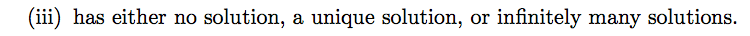
\includegraphics[width=400pt]{img/oxford-prelims-2017-A-2-1-3.png}
\end{mdframed}

Suppose $Ax = b$ has $n > 1$ solutions and let the first two such solutions be
$x_1$ and $x_2$. Then there are uncountably infinitely many solutions, since
for all $\alpha \in \R$
\begin{align*}
A\Big(x_1 + \alpha (x_2 - x_1)\Big) = Ax_1 + \alpha(Ax_2 - Ax_1) = b + \alpha(b - b) = b.
\end{align*}

\newpage
\subsection*{} % 2.b
\begin{mdframed}
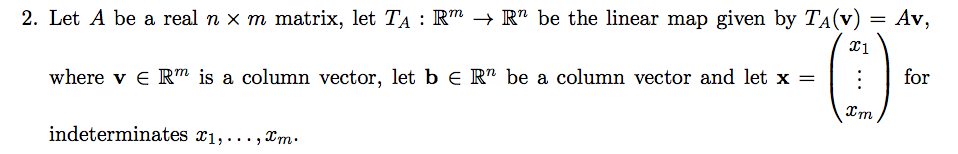
\includegraphics[width=400pt]{img/oxford-prelims-2017-A-2-2-0.png}\\
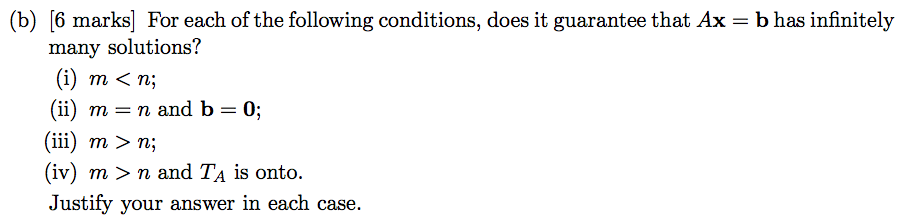
\includegraphics[width=400pt]{img/oxford-prelims-2017-A-2-2.png}
\end{mdframed}

\begin{table}[h]
  \centering
  \begin{tabular}{|c|c|c|c|}
    $          $ & $\Im < \Cod$      & $\Im = \Cod$   & $\Im > \Cod$\\
    \hline
    $\Dom < \Im$ & Impossible        & Impossible     & Impossible  \\
    $\Dom = \Im$ & 0 or 1 (A)        & 1 (B)          & Impossible  \\
    $\Dom > \Im$ & 0 or $\infty$ (C) & $\infty$ (D)   & Impossible  \\
  \end{tabular}
\end{table}

\textbf{(i)} $m < n$. \textbf{No}: case A or C.

% We have $\dim(\Dom T_A) < \dim(\Cod T_A)$. It is possible that
% $\dim(\Dom T_A) \leq \dim(\Im T_A)$ in which case there will not be infinitely
% many solutions.

\textbf{(ii)} $m = n$ and $\vec b = \vec 0$. \textbf{No}: case B or C.

% We know that $\vec b \in \Im T_A$, since $\vec b = \vec 0$. However, it is
% possible that $A$ is invertible. In that case there will be exactly one
% solution for all $b$. (Otherwise, there are infinitely many solutions.)

\textbf{(iii)} $m > n$. \textbf{No}: case A, C or D

% It is possible that $\dim(\Im T_A) < n$, in which case it is possible that
% $b \notin \Im T_A$, in which case there are zero solutions. (But if
% $b \in \Im T_A$ then there are infinitely many solutions.)

\textbf{(iv)} $m > n$ and $T_A$ is onto. \textbf{Yes}: case D

\begin{lemma*}
  $Ax = b$ has infinitely many solutions for all $b \in \Cod T_A$ if and only
  if $\dim(\Dom T_A) > \dim(\Im T_A)$
\end{lemma*}

[Either the map is from a higher dimensional space to a lower dimensional
space, or the image is a lower dimensional subspace.]


\subsection*{} % 2.c
\begin{mdframed}
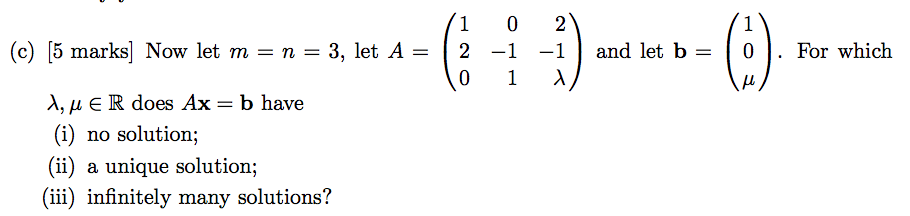
\includegraphics[width=400pt]{img/oxford-prelims-2017-A-2-3.png}
\end{mdframed}

Could be case B (1 solution) or C (infinite solutions).

\textbf{(i)} Impossible

\newpage
\begin{mdframed}
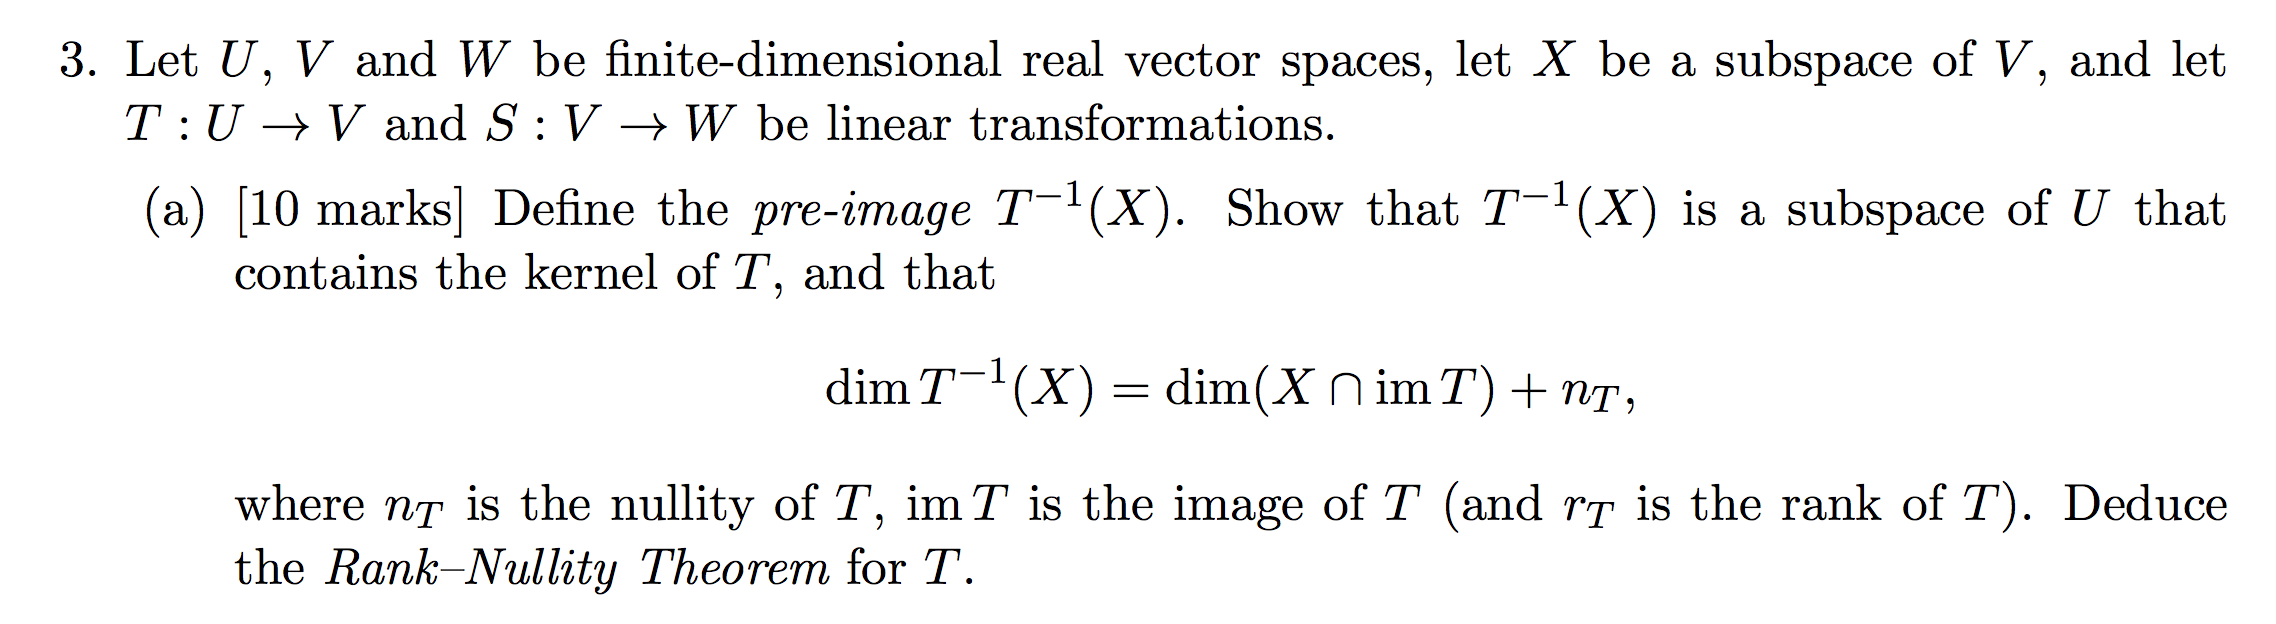
\includegraphics[width=400pt]{img/oxford-prelims-2017-A-3-1.png}
\end{mdframed}

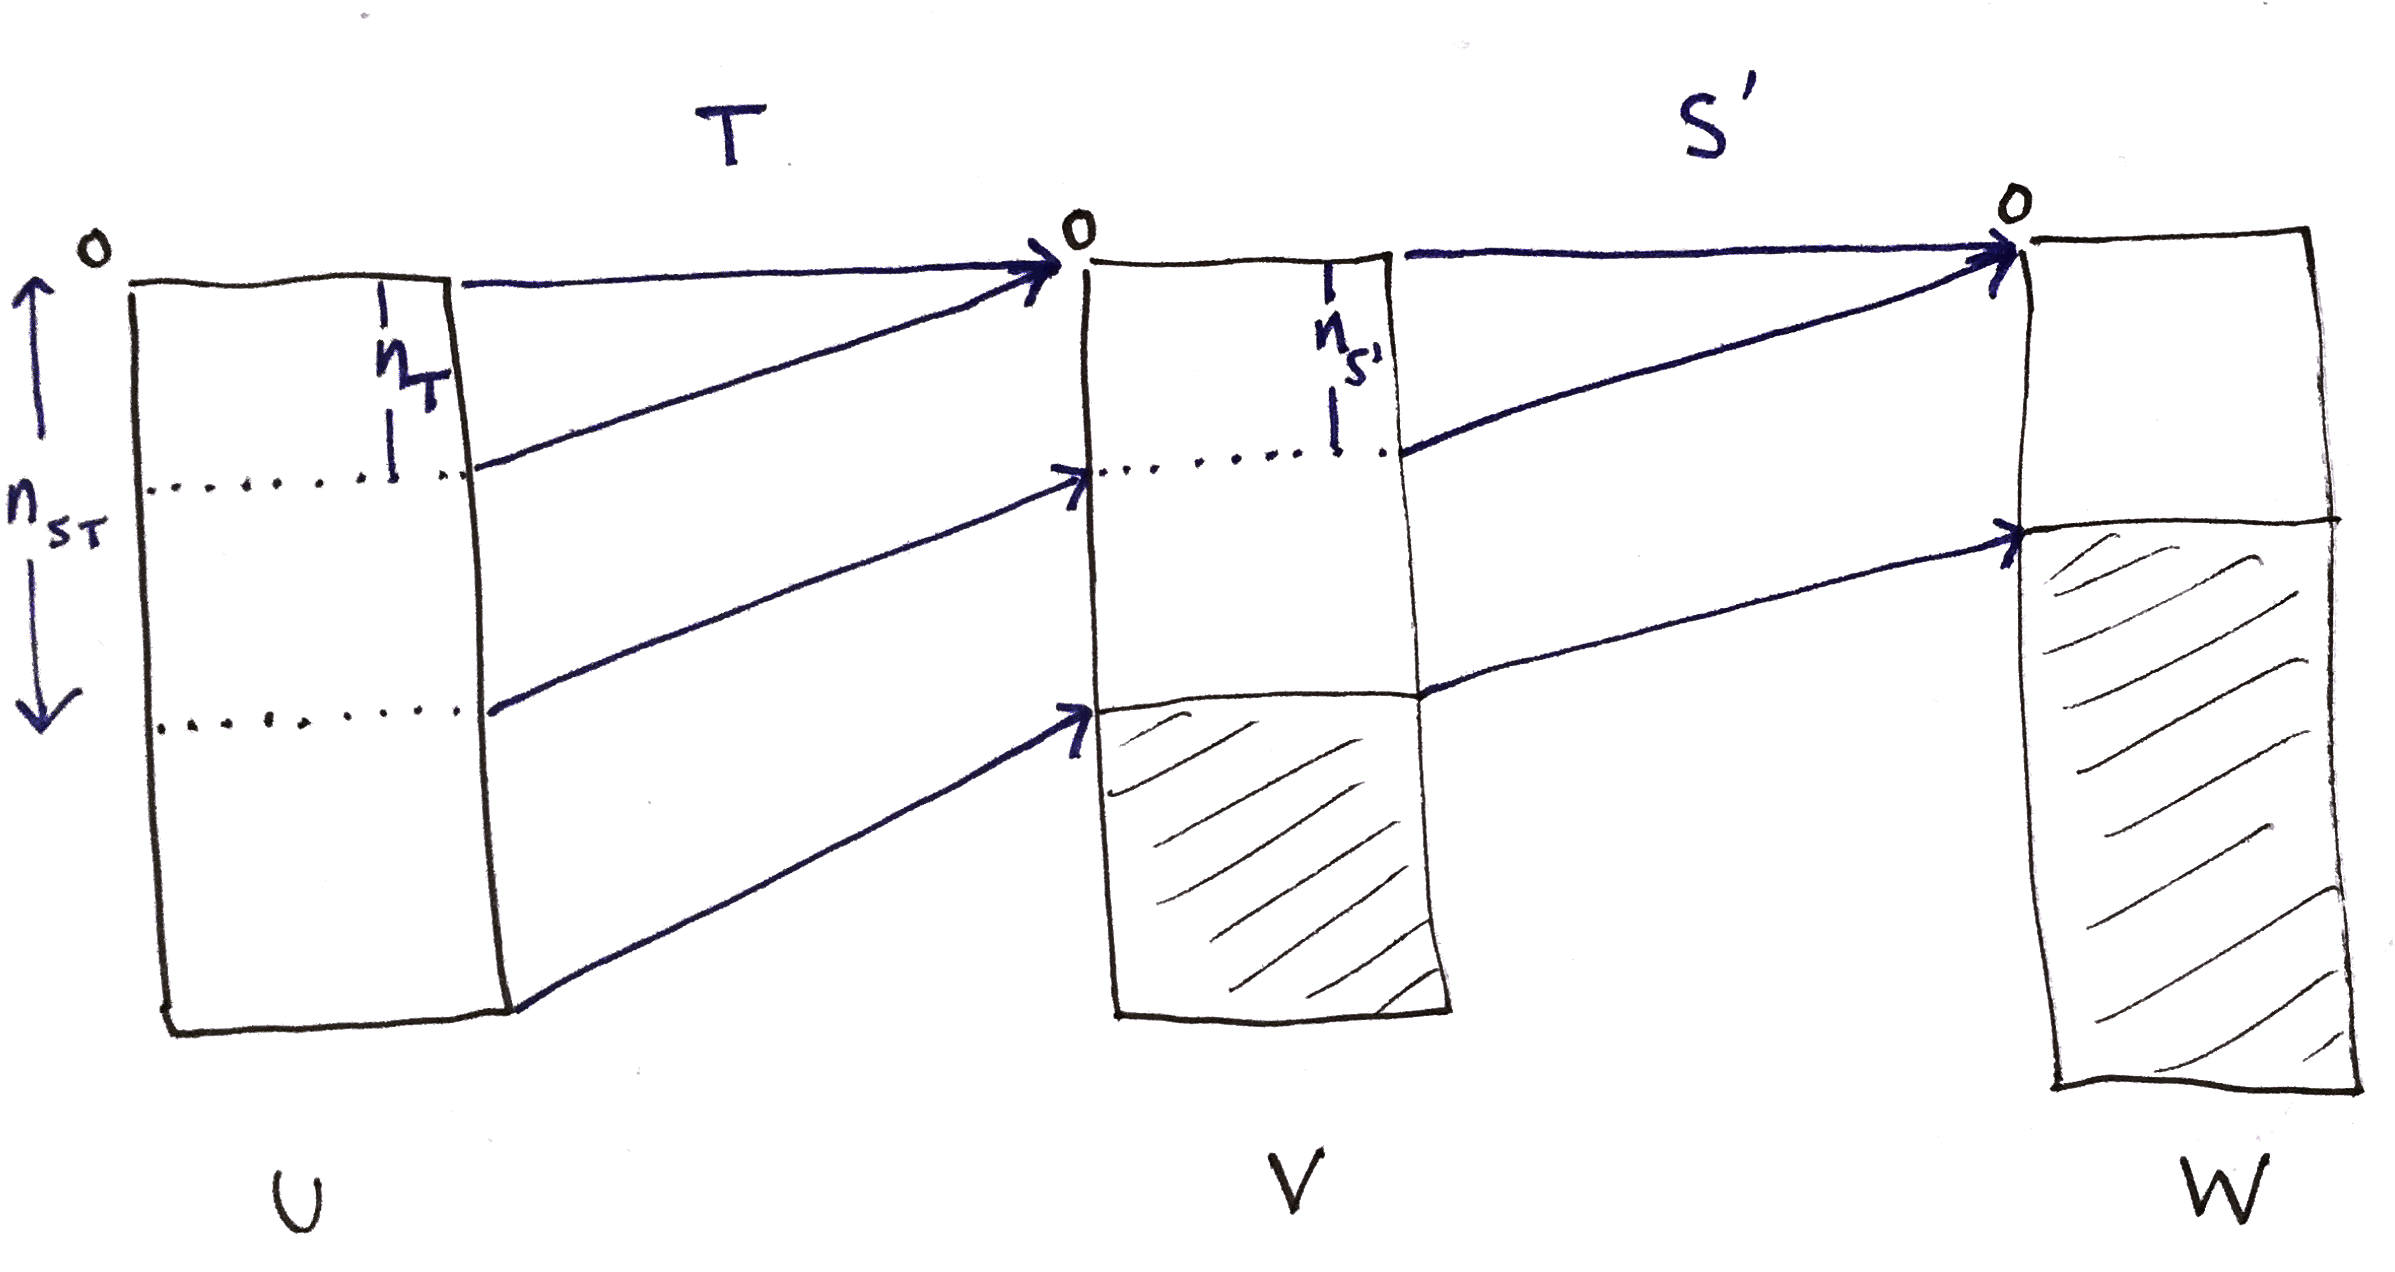
\includegraphics[width=300pt]{img/oxford-prelims-2017-A-3-diagram.png}

\begin{definition*}
The pre-image of $X$ is $T^\1(X) := \{u ~|~ T(u) \in X\}$.
\end{definition*}

\begin{claim*}
  $T^\1(X)$ is a subspace of $U$ that contains $\Ker T$.
\end{claim*}

\begin{proof}
  Note that $0_V \in X$, since $X$ is a subspace of $V$. Therefore
  $\Ker T \subseteq T^\1(X)$.

  To show that $T^\1(X)$ is a subspace of $U$ we must show that it is a subset
  of $U$, that it contains the zero vector, and that it is closed under taking
  linear combinations.

  $T^\1(X)$ is a subset of $U$ by definition of pre-image.

  $T$ is linear, therefore $T(0_U) = 0_V$, therefore $0_U \in T^\1(X)$.

  Let $u_1, \ldots, u_n \in T^\1(X)$ and for $i=1,\ldots, n$ let
  $x_i = T(u_i)$. Consider the linear combination $\sumin \lambda_iu_i$ for
  scalars $\lambda_i$. We have
  $T\Big(\sumin \lambda_iu_i\Big) = \sumin \lambda_ix_i \in X$ by the linearity
  of $T$ and by the fact that $X$ is a subspace. Therefore $T^\1(X)$ is closed
  under taking linear combinations.
\end{proof}

\newpage
\begin{claim*}
  $\dim T^\1(X) = \dim\(X \cap \Im T\) + n_T$
\end{claim*}

\begin{lemma}\label{subspace-basis-extension}
  Let $U$ be a subspace of a finite-dimensional vector space $V$. Then every
  basis of $U$ can be extended to be a basis of $V$. I.e. if $v_1, \ldots, v_m$
  is a basis for $U$, then there exists a basis
  $v_1, \ldots, v_m, v_{m+1}, \ldots, v_n$ of $V$.
\end{lemma}

\begin{lemma}\label{transformed-basis-spans-image}
  Let $U, V$ be vector spaces, let $u_1, \ldots, u_n$ span $U$ and let
  $T:U \to V$ be a linear transformation. Then $T(u_1), \ldots, T(u_n)$ spans
  $V$.
\end{lemma}

\begin{proof}
  Let $T^*: \(T^\1(X)\) \to \(X \cap \Im T\)$ be the restriction of $T$ to $T^\1(X)$.

  From above we have $\Ker T \subseteq T^\1(X)$, therefore $\Ker T = \Ker T^*$
  and $n_T = n_{T^*}$.

  Choose a basis $u_1, \ldots, u_{n_T}$ for $\Ker T^*$ and let
  $n = \dim T^\1(X)$.

  From Lemma \ref{subspace-basis-extension}, this basis can be extended to a
  basis $u_1, \ldots, u_{n_T}, u_{n_T+1}, \ldots, u_n$ of $T^\1(X)$.

  From Lemma \ref{transformed-basis-spans-image},
  $T^*(u_1), \ldots, T^*(u_{n_T}), T^*(u_{n_T+1}), \ldots, T^*(u_n)$ spans
  $\Im T^*$.

  Moreover, $T^*(u_{n_T+1}), \ldots, T^*(u_n)$ spans $\Im T^*$, since
  $T^*(u_1) = \ldots = T^*(u_{n_T}) = 0_V$.

  Suppose that $T^*(u_{n_T+1}), \ldots, T^*(u_n)$ are linearly independent.

  Then they are a basis for $\Im T^*$ and we have
  $r_{T^*} := \dim(\Im T^*) = n - n_T$.

  Note that $\Im T^* = X \cap \Im T$, and recall that $n := \dim T^\1(X)$.

  So we have $\dim T^\1(X) = \dim\(X \cap \Im T\) + n_T$ as required.

  It remains to show that $T^*(u_{n_T+1}), \ldots, T^*(u_{n_T+r_{T^*}})$ are linearly
  independent.

  % Rename and relabel these as follows: for $i = 1, \ldots, r_{T^*}$, let
  % $x_i = u_{n_T + i}$.

  Consider an arbitrary linear dependence relation
  $\sum_{i=1}^{r_{T^*}} \lambda_iT^*(u_{n_T + i}) = 0_V$, for some scalars
  $\lambda_i, \ldots, \lambda_{r_{T^*}}$

  Since $T^*$ is linear, we have
  $T^*\Big(\sum_{i=1}^{r_{T^*}} \lambda_i(u_{n_T + i})\Big) = 0_V$ and hence
  $\sum_{i=1}^{r_{T^*}} \lambda_iu_{n_T+i} \in \Ker T^*$.

  Therefore, using the basis for $\Ker T^*$, we have
  $\sum_{i=1}^{r_{T^*}} \lambda_iu_{n_T+i} = \sum_{i=1}^{n_T} \gamma_iu_i$, for
  some scalars $\gamma_i, \ldots, \gamma_{r_{T^*}}$.

  Therefore $\sum_{i=1}^{n_T+r_{T^*}}\beta_iu_i = 0$, where each $\beta_i$ is
  either $\lambda_i$ or $-\gamma_i$. But since the $u_i$ are a basis of
  $T^\1(X)$ they are linearly independent, hence all the $\beta_i$ are zero,
  and so $\lambda_i = 0$ for all $i \in \{1, \ldots, r_{T^*}\}$.

  Therefore $T^*(u_{n_T+1}), \ldots, T^*(u_{n_T+r_{T^*}})$ are linearly
  independent.
\end{proof}

\newpage
\begin{mdframed}
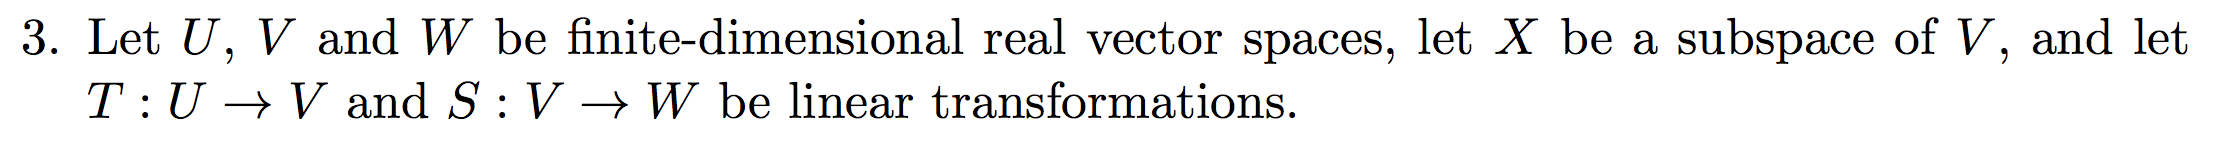
\includegraphics[width=400pt]{img/oxford-prelims-2017-A-3-0.png}\\
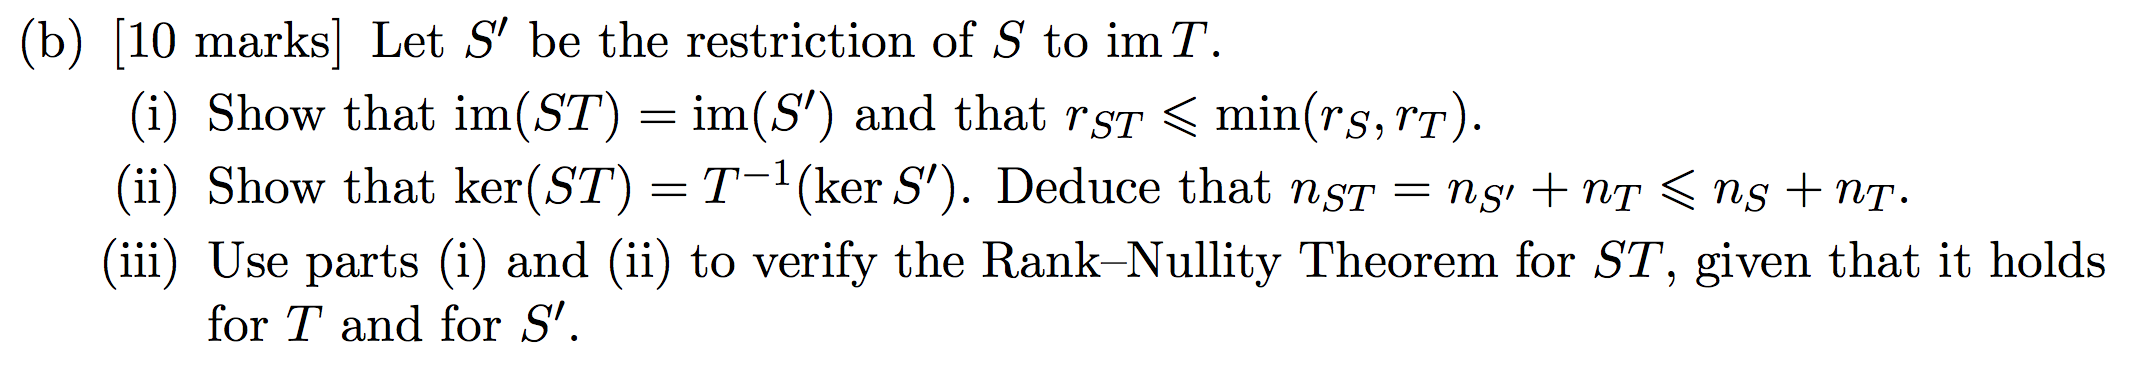
\includegraphics[width=400pt]{img/oxford-prelims-2017-A-3-2.png}
\end{mdframed}
% $\Im ST := \{w ~|~ \exists u: S(T(u)) = w\}$
% $\Im S' := \{w ~|~ \exists v \in \Im T: S(v) = w\}$

\textbf{(i)}

\begin{claim*}
  $\Im ST = \Im S'$.
\end{claim*}
\begin{proof}
For the forwards direction, let $w \in \Im ST$. Then $\exists u \in U$ such
that $S(T(u)) = w$. Since $T(u) \in \Im T$, we have $\exists v \in \Im T$
such that $S(v) = w$. Therefore $w \in \Im S'$.

For the reverse direction, let $w \in \Im S'$. Then $\exists v \in \Im T$ such
that $S(v) = w$. Therefore $\exists u \in U$ such that $S(T(u)) = w$. Therefore
$w \in \Im ST$.
\end{proof}

\begin{claim*}
  $r_{ST} \leq \min\(r_S, r_T\)$.
\end{claim*}
\begin{proof}
  $\Im S'$ is a subspace of $\Im S$\footnote{
    $\Im S'$ is a subset of $\Im S$ and contains $0_W$. Consider
    $\sumin \lambda_iw_i$ for $w_i \in \Im S'$ and scalars $\lambda_i$. For
    each $w_i$ let $u_i \in \Im T$ be such that $S(u_i) = w_i$. Then
    $\Big(\sumin \lambda_i u_i\Big) \in \Im T$ and
    $\sumin \lambda_i w_i = \sumin \lambda_i S(u_i) = S\Big(\sumin \lambda_i
    u_i\Big)$. Therefore $\Im S'$ is a subspace of $\Im S$.
  }, therefore $r_{S'} \leq r_S$ by Lemma \ref{subspace-basis-extension}. Since
  $\Im S' = \Im ST$, we have $r_{ST} \leq r_S$.

Let $v_1, \ldots, v_{r_T}$ be a basis for $\Im T$. From Lemma
\ref{transformed-basis-spans-image} we have $S(v_1), \ldots, S(v_{r_T})$ span
$\Im S' = \Im ST$. Therefore $r_{ST} \leq r_T$.

Therefore $r_{ST} \leq \min\(r_S, r_T\)$.
\end{proof}

\textbf{(ii)}

\begin{claim*}
  $\Ker ST = T^\1\(\Ker S'\)$
\end{claim*}

\begin{proof}~\\
  $u \in \Ker ST \iff S'(T(u)) = 0_W \iff T(u) \in \Ker S' \iff u \in T^\1\(\Ker S'\)$.
\end{proof}

\newpage
\begin{claim*}
  $n_{ST} = n_{S'} + n_T \leq n_S + n_T$.
\end{claim*}

\begin{proof}
  Note that $\Ker T$ is a subspace of $\Ker ST$.

  Let $u_1, \ldots, u_{n_T}$ be a basis for $\Ker T$.

  By Lemma \ref{subspace-basis-extension}, this can be extended to a basis
  $u_1, \ldots, u_{n_T}, u_{n_T + 1}, \ldots, u_{n_{ST}}$ of
  $\Ker ST = T^\1\(\Ker S'\)$.

  By Lemma \ref{transformed-basis-spans-image},
  $T(u_1), \ldots, T(u_{n_T}), T(u_{n_T + 1}), \ldots, T(u_{n_{ST}})$ spans
  $\Ker S'$.

  However $T(u_1) = T(u_2) = \ldots = T(u_{n_T}) = 0_V$, therefore
  $T(u_{n_T + 1}), \ldots, T(u_{n_{ST}})$ also spans $\Ker S'$.

  Therefore $n_{S'} \leq n_{ST} - n_T$.

  In order to prove that this is an equality, we need to show that
  $T(u_{n_T + 1}), \ldots, T(u_{n_{ST}})$ are linearly independent. This
  argument procedes in the usual manner:

  Suppose there exist scalars $\lambda_{n_T+1}, \ldots, \lambda_{n_{ST}}$ such
  that $\sum_{i=n_T+1}^{n_{ST}} \lambda_i T(u_{i}) = 0_V$. Since $T$ is linear
  we have $T\Big(\sum_{i=n_T+1}^{n_{ST}} \lambda_i u_{i}\Big) = 0_V$, therefore
  $\Big(\sum_{i=n_T+1}^{n_{ST}} \lambda_i u_{i}\Big) \in \Ker T$.

  Using our basis for $\Ker T$, we have that there exist scalars
  $\gamma_i, \ldots, \gamma_{n_T}$ such that
  $\sum_{i=n_T+1}^{n_{ST}} \lambda_i u_{i} = \sum_{i=1}^{n_T} \gamma_i u_i$. In
  other words, $\sum_{i=1}^{n_{ST}} \beta_i u_i = 0_U$, where
  $\beta_i = \gamma_i$ if $i < n_T$, otherwise $\beta_i = \lambda_i$.

  But $u_1, \ldots, u_{n_{ST}}$ are linearly independent. So we see that
  \begin{align*}
    \sum_{i=n_T+1}^{n_{ST}} \lambda_i T(u_{i}) = 0_V
    \implies
    \lambda_{n_T+1} = \lambda_{n_T+2} = \ldots = \lambda_{n_{ST}} = 0.
  \end{align*}

  So $T(u_{n_T + 1}), \ldots, T(u_{n_{ST}})$ are linearly independent, and
  therefore are a basis for $\Ker S'$.

  Therefore $n_{S'} = n_{ST} - n_T$, or equivalently, $n_{ST} = n_{S'} + n_T$,
  as required.

  Finally, $\Ker S'$ is a subspace of $\Ker S$, therefore $n_{S'} \leq n_S$ by
  Lemma \ref{subspace-basis-extension}.

  Therefore $n_{ST} = n_{S'} + n_T \leq n_S + n_T$, as required.
\end{proof}

\newpage
\begin{mdframed}
\includegraphics[width=400pt]{img/oxford-prelims-2017-A-3-0.png}\\
\includegraphics[width=400pt]{img/oxford-prelims-2017-A-3-2.png}
\end{mdframed}
\includegraphics[width=300pt]{img/oxford-prelims-2017-A-3-diagram.png}\\
\textbf{(iii)}

\begin{claim*}
  $\dim U = r_{ST} + n_{ST}$.
\end{claim*}

\begin{proof}
  Let $d = \dim U$.

  We need to show that $r_{ST} = d - n_{ST}$, as the diagram suggests is true.

  Long-winded way, similar to previous:

  Let $u_1, \ldots, u_{n_{ST}}$ be a basis of $\Ker ST$.

  We can extend this to a basis
  $u_1, \ldots, u_{n_{ST}}, u_{n_{ST} + 1}, \ldots, u_d$ of $U$, by Lemma
  \ref{subspace-basis-extension}.

  As before, we conclude that $u_{n_{ST} + 1}, \ldots, u_d$ span $r_{ST}$,
  since $u_1, \ldots, u_{n_{ST}}$ are in the kernel of $ST$.

  And as before we conclude that, moreover, $u_{n_{ST} + 1}, \ldots, u_d$ are
  linearly independent.

  Thus we conclude that $r_{ST} = \dim U - n_{ST}$, as required.
\end{proof}

\newpage
\begin{mdframed}
\includegraphics[width=400pt]{img/oxford-prelims-2017-A-4-1.png}
\end{mdframed}
\textbf{(i)}
\begin{definition*}
  The \textbf{characteristic polynomial} $\chi_T$ of $T$ is
  $\det(A - \lambda I)$, where $A$ is the matrix of $T$ with respect to some,
  initial and final, basis of $V$.
\end{definition*}

This is well-defined because:

\begin{claim*}
  Let $A$ be a matrix of $T$ with respect to initial and final basis $B$, and
  let $A'$ be a matrix of $T$ with respect to initial and final basis
  $B'$. Then $\det(A - \lambda I) = \det(A' - \lambda I)$.
\end{claim*}

\begin{proof}
  This follows from the fact that the determinant of $T$ does not depend on the
  choice of basis.

  Let $P$ be the change-of-basis matrix, so that $A' = P^\1AP$. Then
  \begin{align*}
    \det(A' - \lambda I) &= \det(P^\1AP - \lambda I)\\
                         &= \det(P^\1AP - P^\1 P \lambda I)\\
                         &= \det(P^\1\(A - \lambda I\)P)\\
                         &= \det(P^\1)\det(A - \lambda I)\det(P)\\
                         &= \det(A - \lambda I)
  \end{align*}
\end{proof}

\textbf{(ii)}
\begin{definition*}
  A scalar $\lambda$ is an \textbf{eigenvalue} of $T$ if there exists a
  non-zero vector $v \in V$ such that $Tv = \lambda v$. In that case $v$ is an
  \textbf{eigenvector} of $T$.
\end{definition*}

\begin{definition*}
  The \textbf{eigenspace} $E_\lambda$ is the set of all vectors $v$ for which
  $Tv = \lambda v$. Equivalently, it is $\Ker(T - \lambda I)$.
\end{definition*}

\begin{claim*}
  $E_\lambda$ is a subspace of $V$.
\end{claim*}

\begin{proof}
  Clearly $E_\lambda \subseteq V$. Also, $0_V \in E_\lambda$.

  Let $v_1, v_2 \in E_\lambda$ and let $\gamma$ be a scalar from the
  field. Then
  $$
  T(v_1 + \gamma v_2) =
  T(v_1) + \gamma T(v_2) =
  \lambda v_1 + \lambda\gamma v_2 =
  \lambda(v_1 + \gamma v_2).
  $$
  Therefore the eigenspace $E_\lambda$ is a subspace by the Subset Test.
\end{proof}

I think there's a non-trivial point here: if two eigenvectors have the same
eigenvalue, the linearity of the transformation means that all vectors in their
span are also eigenvectors in the same eigenspace. I.e. the only way to have
distinct eigenspaces is

\begin{claim*}
  $E_\lambda \cap E_\mu = \{0\}$.
\end{claim*}

\begin{proof}
  Let $v \neq 0_V \in E_\lambda$. Suppose $v \in E_\mu$. Then
  $Tv = \lambda v = \mu v$, therefore $(\lambda - \mu)v = 0$. Since
  $\mu \neq \lambda$ and $v \neq 0_V$, this is a contradiction, proving that
  $E_\lambda \cap E_\mu = \{0\}$.
\end{proof}

\textbf{(iii)}\\
\begin{proof}
  The following statements are equivalent:

  $\lambda$ is an eigenvalue of $T$.

  $\exists v \neq 0_V$ such that $Tv = \lambda v$.

  $\exists v \neq 0_V$ such that $\(T - \lambda I\)v = 0_V$.

  $\Ker(T - \lambda I) \neq \{0_V\}$.

  $T - \lambda I$ is non-invertible.

  $\det(T - \lambda I) = 0$.

  $\chi_T(\lambda) = 0$.
\end{proof}

\newpage
\begin{mdframed}
\includegraphics[width=400pt]{img/oxford-prelims-2017-A-4-2.png}
\end{mdframed}

Suppose $T^2 = I$. Then $T = T^\1$. Therefore $\det T = \pm 1$.

$T^\1$ exists, therefore $T$ is full rank, therefore $T$ has 3 linearly
independent eigenvectors.

Let $v_1, v_2, v_3$ be linearly independent eigenvectors of $T$.

Then $v_1, v_2, v_3$ are a basis of $T$ and all matrices of $T$ with respect to
this basis are diagonal.

Rescale $v_1, v_2, v_3$ such that the diagonal entries
$\lambda_1, \lambda_2, \lambda_3$ each have magnitude 1.

\red{TODO}

Let $\lambda_1, \lambda_2, \lambda_3$ be the eigenvalues of $T$.

We have $\lambda_1\lambda_2\lambda_3 = \det T = \pm 1$.

Since $T^2 \neq T$, we have $T \neq I$, therefore at least one of
$\lambda_1, \lambda_2, \lambda_3$ is not equal to 1.


\newpage
\begin{mdframed}
\includegraphics[width=400pt]{img/oxford-prelims-2017-A-4-3.png}
\end{mdframed}


\begin{proof}
  We assume that
  \begin{align*}
    T^3 &= T\\
    T^2 &\neq T\\
    T^2 &\neq \id_V.
  \end{align*}

  Since $\dim V = 3$, we have $n_T \in \{0, 1, 2, 3\}$.

  Suppose $n_T = 0$. Then $T^\1$ exists and we have
  $T^\1T^3 = T^2 = T^\1T = I$, which contradicts one of the
  assumptions. Therefore $n_T \neq 0$.

  Suppose $n_T = 3$. Then $\Im T = \{0\}$. Therefore $T^2 = T$, which
  contradicts one of the assumptions. Therefore $n_T \neq 3$.

  Therefore $n_T \in \{1, 2\}$.
\end{proof}

\begin{proof}
  Suppose $n_T = 2$.

  Let $\{v_1, v_2\}$ be a basis for the nullspace of $T$.

  By the Steinitz Exchange lemma, we can find a vector $v_3$ such that
  $(v_1, v_2, v_3)$ is an ordered basis of $V$. Then the matrix of $T$ with
  respect to this basis is
  \begin{align*}
    \matMMMxNNN{\vline}{\vline}{\vline}
               {T(v_1)}{T(v_2)}{T(v_3)}
               {\vline}{\vline}{\vline} =
    \matMMMxNNN{\vline}{\vline}{\vline}
               {0_V}{0_V}{T(v_3)}
               {\vline}{\vline}{\vline}.
  \end{align*}

  \red{TODO}

\end{proof}

\end{document}
